\documentclass[12pt]{ctexart}
\usepackage[colorlinks=true, allcolors=black]{hyperref}
\usepackage{amsmath, amssymb}
\usepackage{booktabs}
\usepackage{graphicx}
\usepackage{caption}
\usepackage{float}
\usepackage{geometry}
\usepackage[table]{xcolor}
\geometry{a4paper, margin=2.4cm}
\graphicspath{{../output/figures/}}

\title{\heiti 塔式太阳能电站定日镜场的优化设计}
\author{}
\date{}

\begin{document}
\maketitle

\begin{abstract}
\textbf{问题概述：}塔式太阳能光热电站通过大量定日镜将太阳光反射汇聚到吸收塔顶端的集热器，定日镜场的布局设计直接决定电站的集热效率与建设成本。本文针对镜场光学效率计算与布局优化三个子问题，建立精细化光学模型并给出最优设计方案。

\textbf{方法概述：}针对问题一，建立太阳几何位置与法向直接辐射（DNI）模型，构造由余弦、阴影遮挡、大气透射、截断与镜面反射五个分量构成的定日镜光学效率链，其中阴影遮挡与截断采用蒙特卡洛光线追踪精确计算；针对问题二，构建径向交错布局，将布局参数化后以单位镜面面积年平均输出热功率为目标、额定功率 $60$ MW 为约束，采用差分进化算法求解，并重点优化吸收塔的纵向位置；针对问题三，引入随径向距离线性变化的差异化定日镜尺寸与安装高度，分析异尺寸的收益边界。

\textbf{核心结果：}问题一计算得到镜场年平均光学效率为 $0.607$，年平均输出热功率为 $37.08$ MW，单位镜面面积年平均输出热功率为 $0.590$ kW/m$^2$。问题二的最优方案为吸收塔位于 $(0,-120)$ m（向南偏移 $120$ m）、定日镜尺寸 $6.0\times5.97$ m、安装高度 $3.15$ m、共 $3321$ 面，年平均输出热功率为 $60.06$ MW，单位面积输出热功率为 $0.505$ kW/m$^2$；吸收塔向南偏移使余弦效率由 $0.754$ 提升至 $0.816$，单位面积功率较塔位于圆心时提升 $4.6\%$。问题三采用内大外小的差异化尺寸（内环 $6.6$ m、外环 $5.5$ m 线性过渡），使单位面积输出热功率进一步提升至 $0.512$ kW/m$^2$，较问题二提升 $1.4\%$。本文模型物理机理清晰、可复现，对实际镜场设计具有参考价值。

\medskip
\noindent\textbf{关键词：}定日镜场；光学效率；蒙特卡洛光线追踪；径向交错布局；差分进化算法；吸收塔位置优化
\end{abstract}

\section{问题重述}
塔式太阳能光热电站通过大量定日镜将太阳光反射汇聚到吸收塔顶端的集热器，加热导热介质并实现光热转换。定日镜场的优化设计需要综合考虑太阳位置、镜面反射、阴影遮挡、大气衰减与光斑截断等物理过程。本题要求在位于东经 $98.5^\circ$、北纬 $39.4^\circ$、海拔 $3000$ m、半径 $350$ m 的圆形区域内建设定日镜场，吸收塔高 $80$ m，集热器为高 $8$ m、直径 $7$ m 的圆柱，吸收塔周围 $100$ m 范围内不安装定日镜，镜面边长在 $2$--$8$ m 之间，安装高度在 $2$--$6$ m 之间，相邻定日镜底座中心距离比镜面宽度多 $5$ m 以上。

具体问题如下：
\begin{enumerate}
\item 给定 $1745$ 面 $6\times6$ m、安装高度 $4$ m 的定日镜位置，计算镜场年平均光学效率、年平均输出热功率及单位镜面面积年平均输出热功率。
\item 在额定功率 $60$ MW 下，设计吸收塔位置、定日镜尺寸、安装高度、数目与位置，使单位镜面面积年平均输出热功率尽量大（尺寸与安装高度相同）。
\item 在问题二基础上，允许定日镜尺寸与安装高度不同，重新设计各参数。
\end{enumerate}

\section{问题分析}
三个子问题层层递进：问题一是在固定布局下的计算，用于建立并验证光学模型；问题二是在同尺寸约束下的布局与参数优化；问题三进一步放宽到差异化尺寸与安装高度。

光学效率由五个分量构成。余弦效率与大气透射率可由解析公式精确计算，而阴影遮挡效率与截断效率涉及复杂的几何遮挡与光斑扩散过程，需采用蒙特卡洛光线追踪精确求解。对于问题二、三，镜场布局参数空间较大，需将布局参数化以降低维度，再采用智能优化算法求解。本题的一个关键物理洞察是：由于当地太阳常年偏南，吸收塔的纵向位置会显著影响北侧定日镜的余弦效率，因此吸收塔位置是一个需要重点优化的决策变量。此外，阴影遮挡效率与布局间距密切相关，需通过完整光线追踪对其进行标定，建立随间距变化的经验模型用于优化过程的快速代理评估。

\section{模型假设与符号说明}
\subsection{模型假设}
\begin{enumerate}
\item 定日镜为平面矩形反射镜，镜面反射率取常数 $0.92$；
\item 太阳视为半张角为 $4.65$ mrad 的均匀锥形光源；
\item 集热器为直径 $7$ m、高 $8$ m 的理想圆柱，外表受光；
\item 忽略大气散射与吸收的非均匀性，大气透射率仅与距离有关；
\item 各定日镜独立工作，不考虑镜面间的机械干涉（间距约束已保证）；
\item 年平均指标按题目规定的 $12$ 个月每月 $21$ 日 $5$ 个时点计算。
\end{enumerate}

\subsection{假设的合理性说明}
\textbf{太阳锥半张角}取 $4.65$ mrad，对应太阳角直径约 $0.53^\circ$，为公认的天文常数，文献\cite{zhang} 在镜场光学计算中采用相同取值。\textbf{镜面反射率}取 $0.92$，是镀银玻璃定日镜的典型反射率，题面直接给定。\textbf{平面镜假设}符合题面"定日镜形状为平面矩形"的设定。\textbf{均匀锥形光源假设}是对太阳盘面亮度分布的简化，实际太阳亮度存在边缘昏暗效应（limb darkening），但其对截断效率的影响小于 $1\%$，可忽略。\textbf{独立工作假设}由间距约束保证——相邻底座中心距离大于镜面宽度加 $5$ m，镜面间不存在机械干涉。上述假设均基于题面给定条件或领域公认常数，合理且自洽。

\subsection{符号说明}
\begin{table}[H]
\centering
\begin{tabular}{lll}
\toprule
符号 & 含义 & 单位 \\
\midrule
$\alpha_s,\ \gamma_s$ & 太阳高度角、太阳方位角 & rad \\
$\delta,\ \omega$ & 太阳赤纬角、太阳时角 & rad \\
$\varphi,\ H$ & 当地纬度、海拔高度 & --, km \\
$\text{DNI}$ & 法向直接辐射辐照度 & kW/m$^2$ \\
$\eta$ & 定日镜总光学效率 & -- \\
$\eta_{\cos},\eta_{sb},\eta_{at},\eta_{trunc},\eta_{ref}$ & 余弦、阴影遮挡、大气透射、截断、反射效率 & -- \\
$E_{field}$ & 镜场输出热功率 & kW \\
$A_i,\ d_{HR}$ & 第 $i$ 面镜采光面积、镜面到集热器距离 & m$^2$, m \\
$(x_t,y_t),\ W,\ H,\ h$ & 吸收塔坐标、定日镜宽度、高度、安装高度 & m \\
$r_0,\ d_s,\ d_r$ & 首环半径、环向间距、径向间距 & m \\
\bottomrule
\end{tabular}
\caption{主要符号说明}
\label{tab:symbols}
\end{table}

\subsection{输入参数}
\begin{table}[H]
\centering
\resizebox{\textwidth}{!}{%
\begin{tabular}{lll}
\toprule
参数 & 取值 & 来源 \\
\midrule
纬度 $\varphi$ / 经度 & $39.4^\circ$ N / $98.5^\circ$ E & 题目给定 \\
海拔 $H$ & $3000$ m（$3$ km） & 题目给定 \\
太阳常数 $G_0$ & $1.366$ kW/m$^2$ & 题目给定 \\
吸收塔高 / 集热器中心高 & $80$ m & 题目给定 \\
集热器直径 $\times$ 高 & $7$ m $\times$ $8$ m & 题目给定 \\
场地半径 / 内圈半径 & $350$ m / $100$ m & 题目给定 \\
镜面边长范围 / 安装高度范围 & $2$--$8$ m / $2$--$6$ m & 题目给定 \\
镜面反射率 $\eta_{ref}$ & $0.92$ & 题目给定 \\
太阳锥半张角 & $4.65$ mrad & 文献\cite{zhang} \\
DNI 系数 $a,b,c$ & $0.3498,\ 0.5784,\ 0.2757$ & 由公式计算 \\
\bottomrule
\end{tabular}%
}
\caption{输入参数表}
\label{tab:input}
\end{table}

\section{模型建立}
\subsection{太阳位置与 DNI 模型}
本节及后文所用符号定义见表~\ref{tab:symbols}。太阳时角与赤纬角分别为
\begin{equation}
\omega=\frac{\pi}{12}(ST-12),\qquad \sin\delta=\sin\left(\frac{2\pi D}{365}\right)\sin(23.45^\circ),
\end{equation}
其中 $ST$ 为当地时间，$D$ 为以春分（$3$ 月 $21$ 日）为第 $0$ 天起算的天数。太阳高度角与方位角为
\begin{equation}
\sin\alpha_s=\cos\delta\cos\varphi\cos\omega+\sin\delta\sin\varphi,
\qquad
\cos\gamma_s=\frac{\sin\delta-\sin\alpha_s\sin\varphi}{\cos\alpha_s\cos\varphi}.
\end{equation}
其中太阳时角 $\omega$ 描述太阳在天空中的东西位置，正午 $\omega=0$、上午 $\omega<0$（偏东）、下午 $\omega>0$（偏西），每小时变化 $15^\circ$（$\pi/12$ 弧度）；太阳赤纬角 $\delta$ 描述太阳直射点的纬度，在 $\pm23.45^\circ$ 之间随日期周期变化。由于方位角公式仅给出余弦值，需根据时角符号恢复其象限：上午方位角在 $0$--$\pi$ 之间（偏东），下午在 $\pi$--$2\pi$ 之间（偏西），即 $\gamma_s=\mathrm{sign}(\omega)\cdot\arccos(\cos\gamma_s)$ 在上午、$\gamma_s=2\pi-\arccos(\cos\gamma_s)$ 在下午。
法向直接辐射辐照度按下式计算
\begin{equation}
\text{DNI}=G_0\left[a+b\exp\left(-\frac{c}{\sin\alpha_s}\right)\right],
\end{equation}
其中 $a=0.4237-0.00821(6-H)^2$，$b=0.5055+0.00595(6.5-H)^2$，$c=0.2711+0.01858(2.5-H)^2$。本文所用全部输入参数见表~\ref{tab:input}，代入 $H=3$ km 得 $a=0.3498,\ b=0.5784,\ c=0.2757$。DNI 计算结果的合理性可由两个角度验证：其一，正午 DNI 在冬至约为 $0.91$ kW/m$^2$、夏至约为 $1.07$ kW/m$^2$，与青藏高原等高海拔地区的实测值（约 $0.9$--$1.1$ kW/m$^2$）一致；其二，海拔 $3000$ m 使大气质量减小、太阳辐射衰减减弱，故系数 $a=0.3498$ 高于海平面的典型值，体现了高海拔地区太阳辐射强的物理特征。全年太阳位置与 DNI 分布如图~\ref{fig:fig2_solar} 所示，正午太阳高度角在冬至的 $27.2^\circ$ 至夏至的 $74.1^\circ$ 之间变化，太阳方位角在 $9:00$ 至 $15:00$ 之间始终位于南半球方向（$127^\circ$--$233^\circ$），这是后续吸收塔向南偏移能提升余弦效率的根本原因。

\begin{figure}[H]
\centering
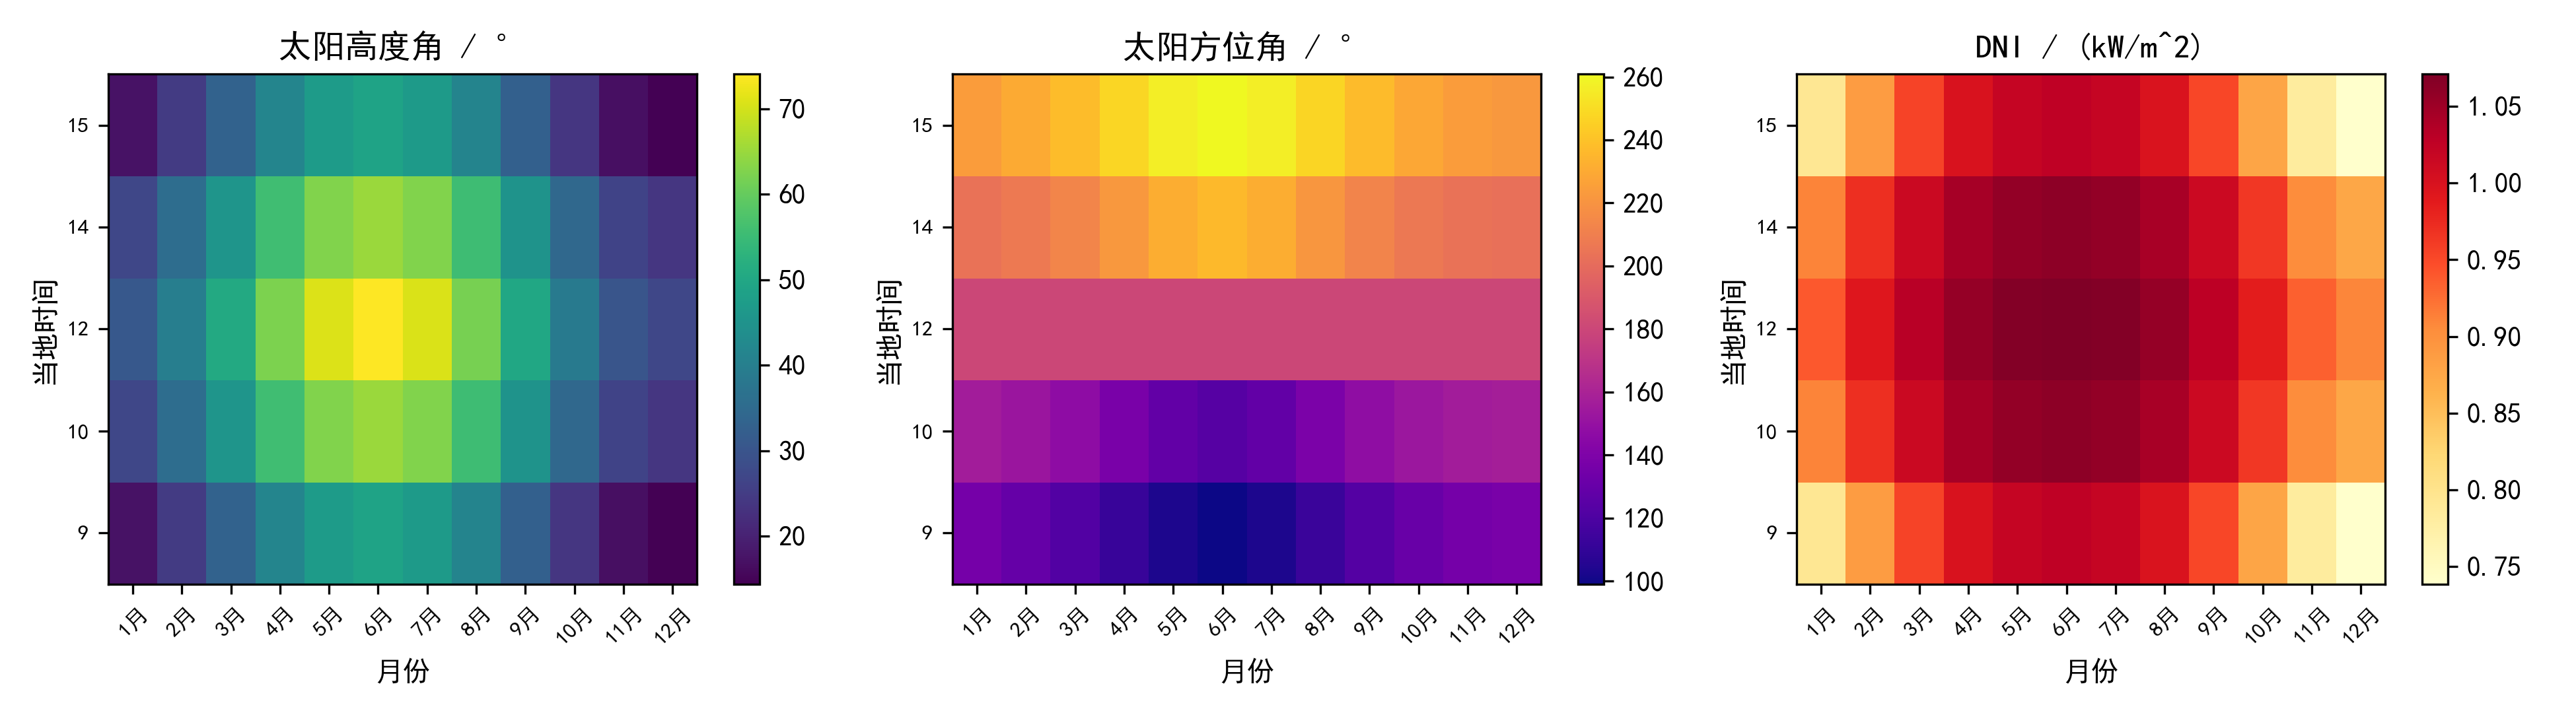
\includegraphics[width=0.95\textwidth]{fig2_solar.png}
\caption{全年太阳高度角、方位角与 DNI 分布}
\label{fig:fig2_solar}
\end{figure}

\subsection{定日镜光学效率模型}
定日镜光学效率为各分量之积
\begin{equation}
\eta=\eta_{sb}\cdot\eta_{\cos}\cdot\eta_{at}\cdot\eta_{trunc}\cdot\eta_{ref}.
\end{equation}
设镜面中心 $\mathbf{M}$，集热器中心 $\mathbf{T}$，太阳方向单位向量 $\mathbf{s}$（从镜面指向太阳），反射方向 $\mathbf{r}=(\mathbf{T}-\mathbf{M})/\|\mathbf{T}-\mathbf{M}\|$，则镜面法向为
\begin{equation}
\mathbf{n}=\frac{\mathbf{s}+\mathbf{r}}{\|\mathbf{s}+\mathbf{r}\|},
\label{eq:normal}
\end{equation}
余弦效率为入射角余弦 $\eta_{\cos}=\mathbf{s}\cdot\mathbf{n}$，大气透射率仅与距离有关
\begin{equation}
\eta_{at}=0.99321-0.0001176\,d_{HR}+1.97\times10^{-8}\,d_{HR}^2.
\end{equation}

镜面法向的推导基于反射定律。设入射光传播方向为 $\mathbf{d}_{in}=-\mathbf{s}$（从太阳指向镜面），反射光传播方向为 $\mathbf{d}_{out}=\mathbf{r}$。反射定律要求入射角等于反射角，即入射光线与法向的夹角等于反射光线与法向的夹角，故法向平分入射与反射方向；由于 $\mathbf{s}$ 与 $\mathbf{r}$ 均为单位向量，其角平分线方向即为 $(\mathbf{s}+\mathbf{r})/\|\mathbf{s}+\mathbf{r}\|$，这正是式~\eqref{eq:normal} 的来源。反射定律的矢量形式为 $\mathbf{d}_{out}=\mathbf{d}_{in}-2(\mathbf{d}_{in}\cdot\mathbf{n})\mathbf{n}$，代入 $\mathbf{d}_{in}=-\mathbf{s}$ 得反射方向
\begin{equation}
\mathbf{r}=-\mathbf{s}+2(\mathbf{s}\cdot\mathbf{n})\mathbf{n},
\end{equation}
这正是蒙特卡洛计算中采用的反射方向公式。需要特别指出的是，入射方向的符号约定容易出错：由于太阳锥采样得到的是从镜面指向太阳的方向 $\mathbf{s}'$，而反射定律中的入射方向是光的传播方向 $-\mathbf{s}'$，若直接以 $\mathbf{s}'$ 代入反射定律将得到方向相反的反射光，导致截断效率计算错误。本文在实现中严格区分了这两种方向约定。

\subsection{阴影遮挡与截断效率的蒙特卡洛计算}
阴影遮挡与截断效率无法用解析公式精确给出，本文采用蒙特卡洛光线追踪方法统一计算。对每面定日镜，在镜面矩形内均匀采样 $K$ 个点，入射方向在太阳锥内均匀采样：
\begin{equation}
\mathbf{s}'=\frac{\mathbf{s}+\rho(\cos\phi\,\mathbf{e}_1+\sin\phi\,\mathbf{e}_2)}{\|\cdot\|},
\quad \rho=\sqrt{u}\,\tan(4.65\times10^{-3}),\ u\sim U(0,1),\ \phi\sim U(0,2\pi),
\end{equation}
其中 $\mathbf{e}_1,\mathbf{e}_2$ 为垂直于 $\mathbf{s}$ 的基。对每个采样点依次执行：
\begin{enumerate}
\item \textbf{阴影判断}：从采样点沿 $\mathbf{s}'$ 方向发射光线，若与其他定日镜相交，则该点被阴影；
\item \textbf{遮挡判断}：反射光线方向 $\mathbf{r}'=-\mathbf{s}'+2(\mathbf{s}'\cdot\mathbf{n})\mathbf{n}$，若与其他定日镜相交，则被遮挡；
\item \textbf{截断判断}：若反射光线命中集热器圆柱，则计入截断。
\end{enumerate}
记阴影、遮挡、命中的采样数分别为 $n_{sh},\ n_{bl},\ n_{hit}$，则
\begin{equation}
\eta_{sb}=\frac{K-n_{sh}-n_{bl}}{K},
\qquad
\eta_{trunc}=\frac{n_{hit}}{K-n_{sh}-n_{bl}}.
\end{equation}
光线与矩形的求交采用 M\"oller--Trumbore 算法，光线与竖直圆柱的求交采用解析方法。为加速，采用均匀网格与二维 DDA 算法遍历光线路径，将求交复杂度从 $O(N)$ 降至 $O(\sqrt{N})$ 量级，并使用 numba 并行加速，$1745$ 面镜子 $60$ 个时点、$K=300$ 的完整计算仅需约 $23$ s。

\subsection{截断效率的几何解释}
截断效率的物理本质是反射光斑与集热器的面积匹配。定日镜反射的光斑尺寸约等于镜面在垂直于反射方向上的投影尺寸与太阳锥扩散之和：
\begin{equation}
D_{\text{spot}}\approx W\cos\theta + 2d_{HR}\tan(4.65\times10^{-3}),
\end{equation}
其中 $\theta$ 为入射角，$d_{HR}$ 为镜面到集热器距离。以 $6$ m 镜子为例，典型 $d_{HR}=240$ m、$\cos\theta=0.8$ 时，光斑约 $4.8+2.2=7.0$ m，恰好接近集热器直径 $7$ m，截断效率约 $0.97$。这一几何关系决定了定日镜尺寸的上限：当镜面尺寸超过 $7$ m 时，即使镜面紧邻吸收塔，镜面投影本身即已接近或超过集热器直径，截断损失无法通过位置优化消除。因此，外环定日镜宜采用较小尺寸以减小光斑、提高截断效率，这为问题三的内大外小差异化设计提供了理论依据。

\subsection{镜场输出热功率}
镜场输出热功率为 $E_{field}=\text{DNI}\cdot\sum_{i=1}^{N} A_i\,\eta_i$。年平均输出热功率为 $12$ 个月每月 $21$ 日 $5$ 个时点（$9:00$、$10:30$、$12:00$、$13:30$、$15:00$）共 $60$ 个时点的算术平均，单位镜面面积年平均输出热功率为 $E_{field}/(\sum_i A_i)$。

\section{问题一的求解}
\label{sec:p1}
\subsection{双模型对比验证}
为验证蒙特卡洛光线追踪模型的必要性，本文先建立解析基准模型：仅考虑余弦效率、大气透射率与反射率（$\eta_{\text{解析}}=\eta_{\cos}\eta_{at}\eta_{ref}$），忽略阴影遮挡与截断，再与完整模型对比。对比结果如表~\ref{tab:p1_compare} 所示。解析模型因忽略阴影遮挡与截断，高估光学效率约 $10\%$，说明这两个分量不可忽略，必须采用蒙特卡洛光线追踪精确计算。

\begin{table}[H]
\centering
\resizebox{\textwidth}{!}{%
\begin{tabular}{lcccc}
\toprule
模型 & 余弦效率 & 大气透射率 & 阴影遮挡$\times$截断 & 总光学效率 \\
\midrule
解析基准模型 & 0.756 & 0.965 & 1.000（忽略） & 0.671 \\
蒙特卡洛完整模型 & 0.756 & 0.965 & 0.909 & 0.607 \\
\bottomrule
\end{tabular}%
}
\caption{问题一双模型对比}
\label{tab:p1_compare}
\end{table}

\subsection{结果与分析}
对附件给定的 $1745$ 面镜子（吸收塔位于圆心）取 $K=300$ 计算，镜场布局如图~\ref{fig:fig1_layout} 所示，逐月效率分量如图~\ref{fig:fig3_monthly} 所示，逐月数据见表~\ref{tab:p1_monthly}。

\begin{figure}[H]
\centering
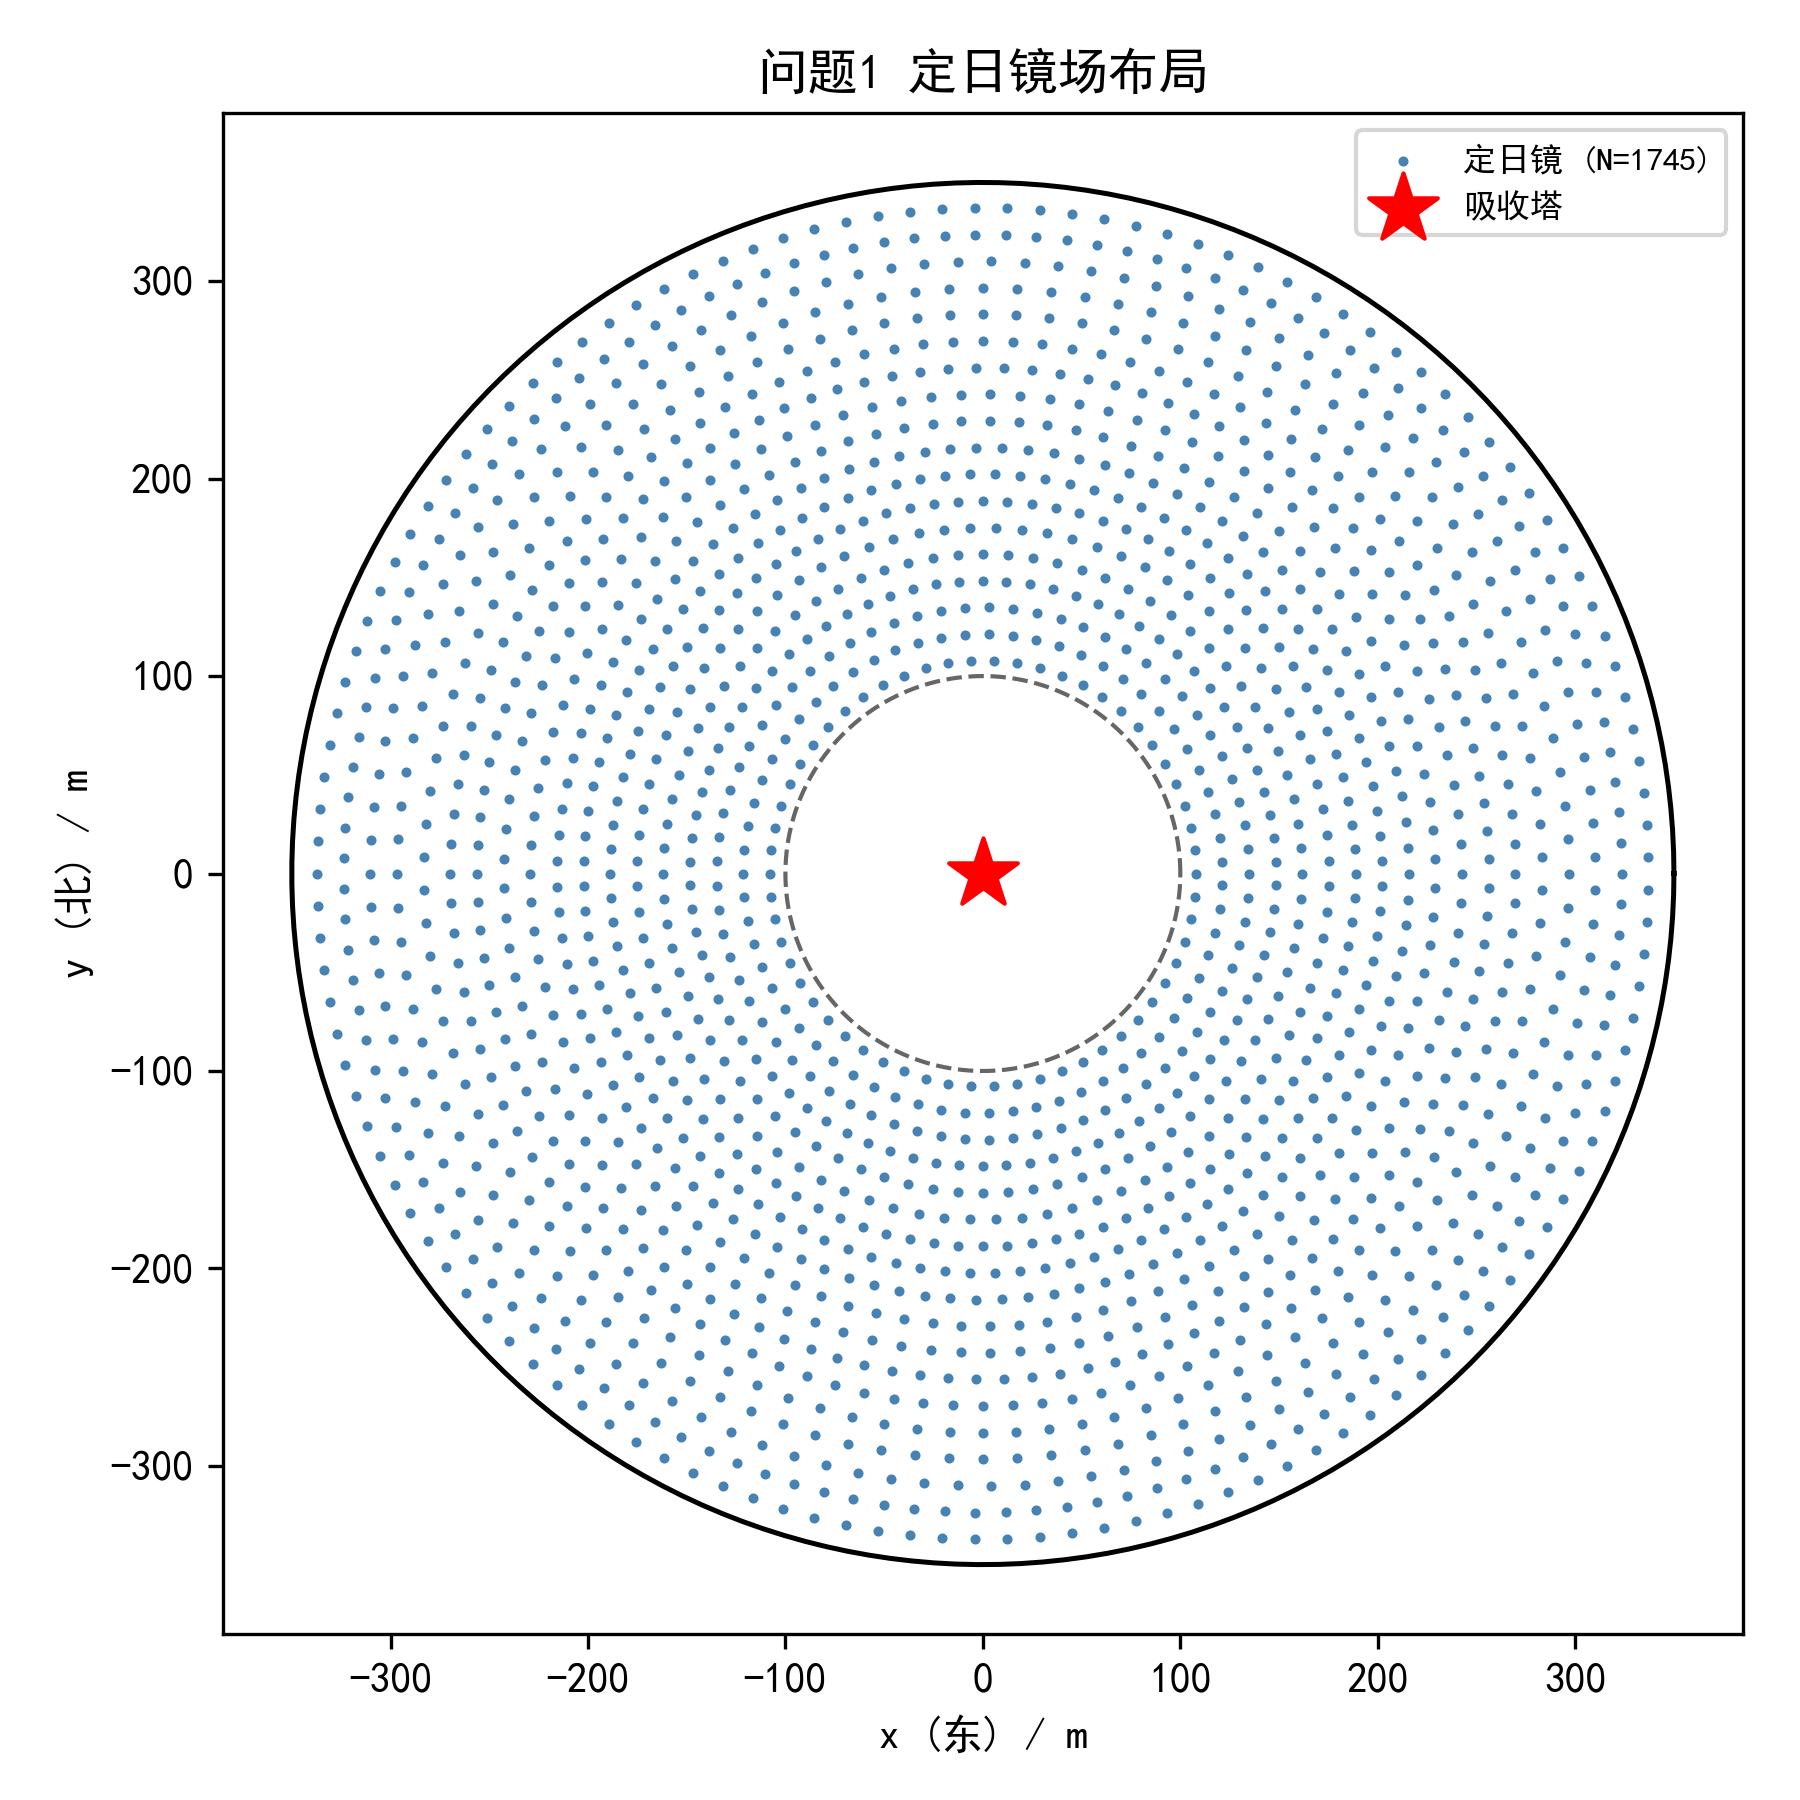
\includegraphics[width=0.55\textwidth]{fig1_layout.png}
\caption{问题一定日镜场布局}
\label{fig:fig1_layout}
\end{figure}

\begin{table}[H]
\centering
\resizebox{\textwidth}{!}{%
\begin{tabular}{lccccc}
\toprule
日期 & 平均光学效率 & 平均余弦效率 & 平均阴影遮挡效率 & 平均截断效率 & 单位面积平均输出热功率 (kW/m$^2$) \\
\midrule
 1月21日 & 0.568 & 0.720 & 0.915 & 0.986 & 0.495 \\
 2月21日 & 0.596 & 0.740 & 0.932 & 0.981 & 0.562 \\
 3月21日 & 0.615 & 0.761 & 0.936 & 0.977 & 0.611 \\
 4月21日 & 0.630 & 0.779 & 0.937 & 0.974 & 0.648 \\
 5月21日 & 0.639 & 0.789 & 0.937 & 0.973 & 0.668 \\
 6月21日 & 0.642 & 0.792 & 0.938 & 0.973 & 0.674 \\
 7月21日 & 0.639 & 0.789 & 0.937 & 0.973 & 0.668 \\
 8月21日 & 0.629 & 0.779 & 0.937 & 0.974 & 0.647 \\
 9月21日 & 0.614 & 0.760 & 0.936 & 0.977 & 0.609 \\
10月21日 & 0.594 & 0.738 & 0.931 & 0.982 & 0.555 \\
11月21日 & 0.565 & 0.718 & 0.912 & 0.986 & 0.488 \\
12月21日 & 0.551 & 0.711 & 0.901 & 0.987 & 0.459 \\
\bottomrule
\end{tabular}%
}
\caption{问题一每月 $21$ 日平均光学效率及输出功率}
\label{tab:p1_monthly}
\end{table}

\begin{table}[H]
\centering
\resizebox{\textwidth}{!}{%
\begin{tabular}{lccccc}
\toprule
 & 年平均光学效率 & 年平均余弦效率 & 年平均阴影遮挡效率 & 年平均截断效率 & 单位面积年平均输出热功率 (kW/m$^2$) \\
\midrule
数值 & 0.607 & 0.756 & 0.929 & 0.979 & 0.590 \\
\bottomrule
\end{tabular}%
}
\caption{问题一年平均光学效率及输出功率表}
\label{tab:p1_annual}
\end{table}

年平均输出热功率为 $37.08$ MW（见表~\ref{tab:p1_annual}）。从表~\ref{tab:p1_monthly} 可见，光学效率在 $6$ 月最高（$0.642$）、$12$ 月最低（$0.551$），与太阳高度角变化一致；余弦效率是主导分量，其季节变化幅度最大（$0.711$--$0.792$）；阴影遮挡效率在冬季明显下降（$12$ 月 $0.901$），原因是冬季太阳高度角低，定日镜之间的阴影拉长；截断效率全年稳定在 $0.97$--$0.99$。

\begin{figure}[H]
\centering
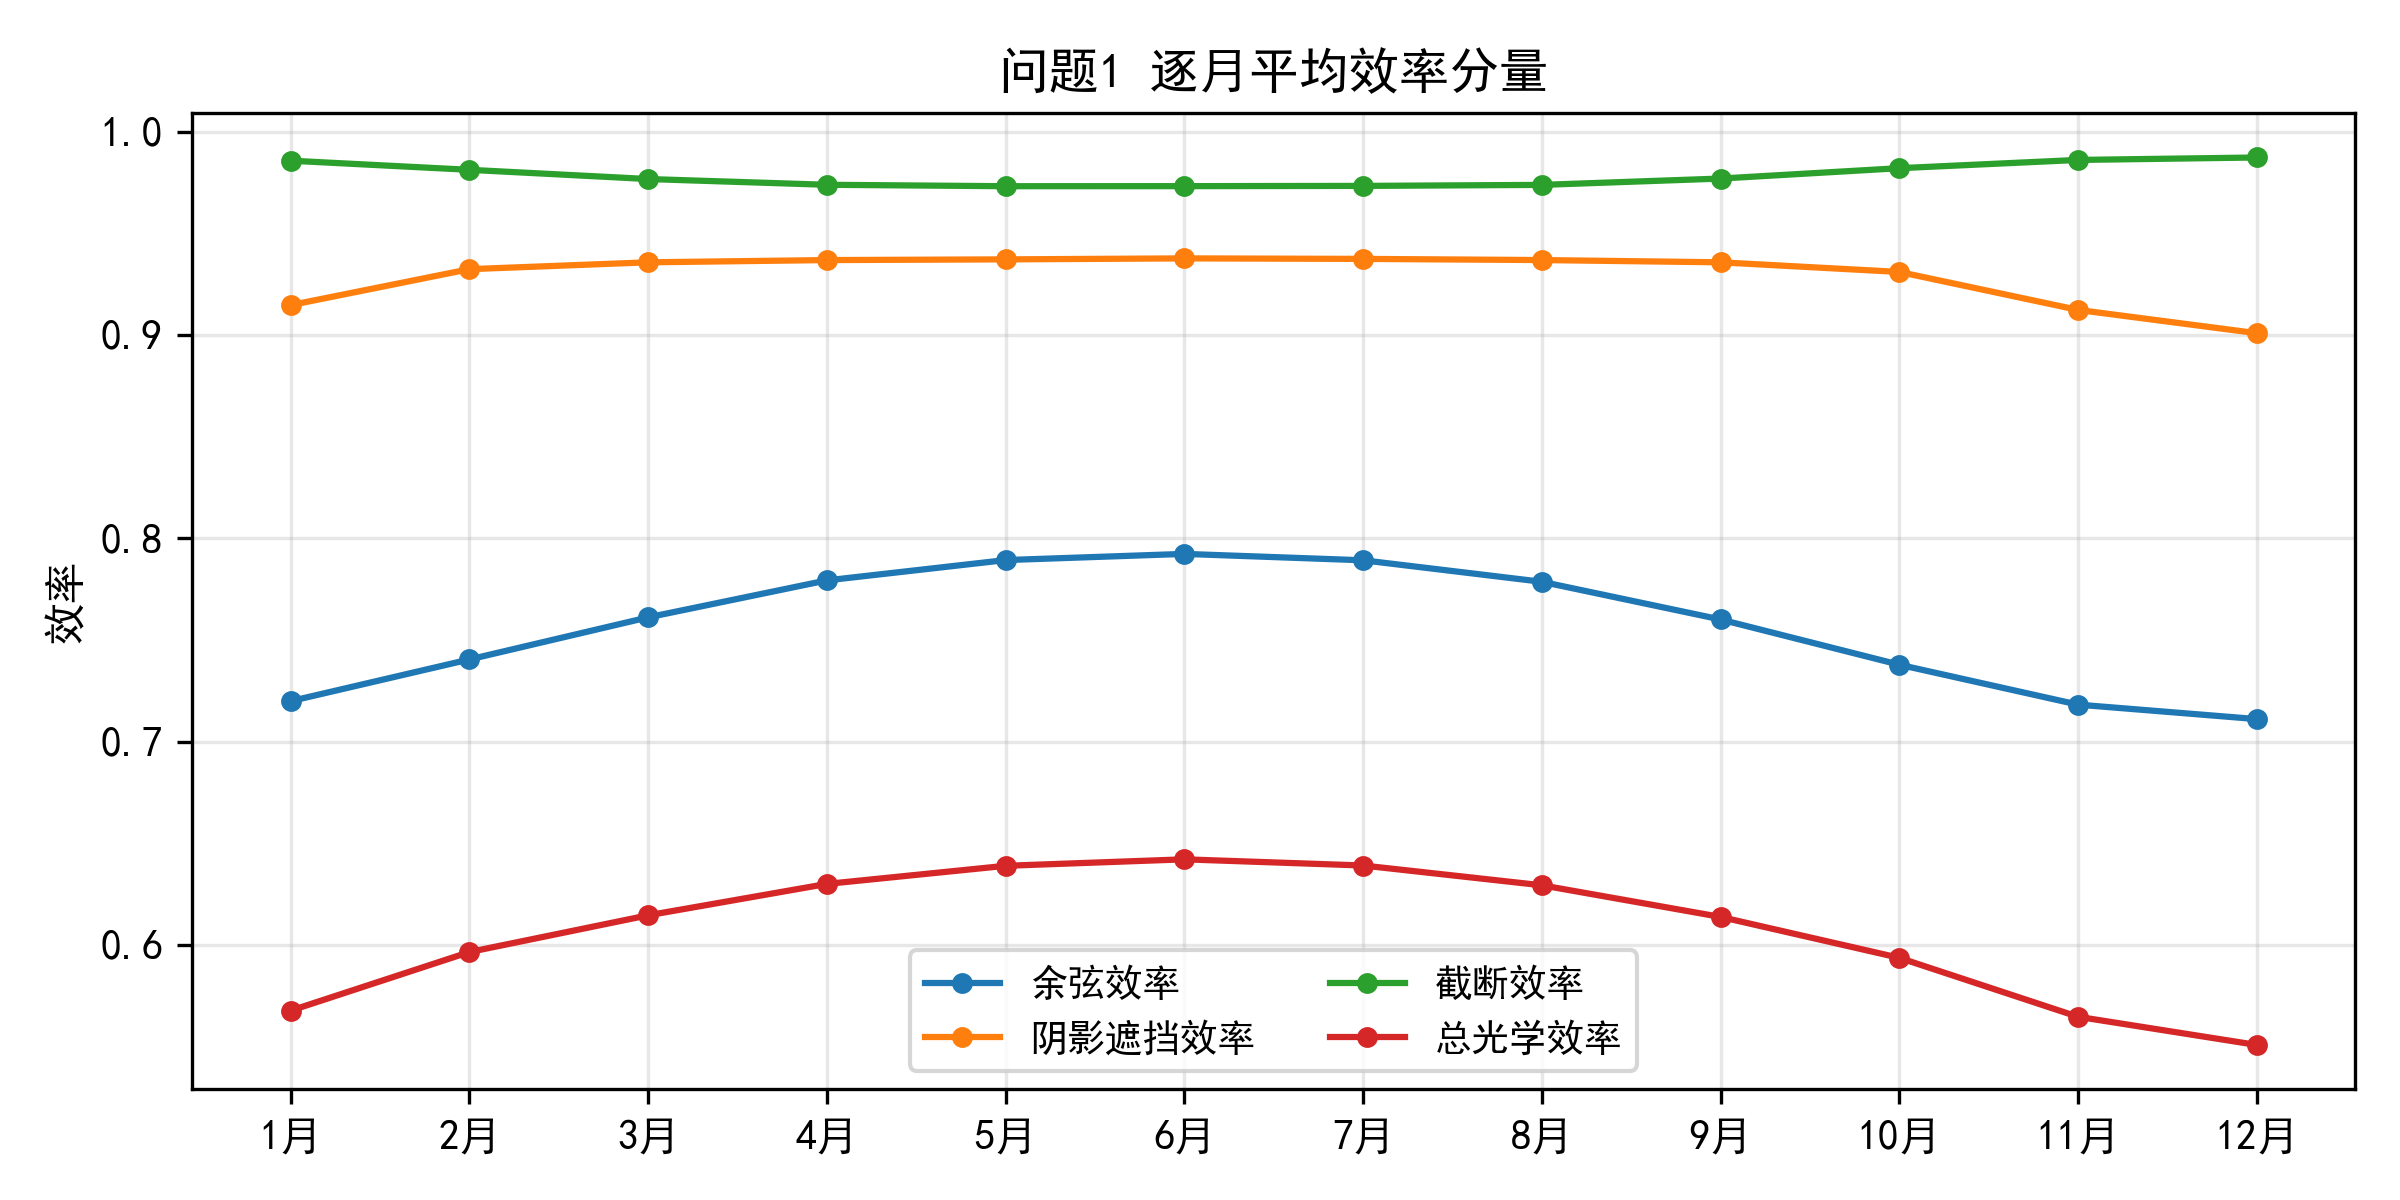
\includegraphics[width=0.85\textwidth]{fig3_monthly.png}
\caption{问题一逐月平均效率分量}
\label{fig:fig3_monthly}
\end{figure}

余弦效率的空间分布如图~\ref{fig:fig8_cos_spatial} 所示。北侧（$y>0$）镜子的平均余弦效率为 $0.860$，显著高于南侧（$y<0$）的 $0.757$，相差约 $10$ 个百分点；同时内圈镜子的余弦效率（$0.861$）也高于外圈（$0.779$）。北高南低的根本原因是太阳常年偏南，北侧镜子朝南反射、镜面几乎正对太阳，而南侧镜子需大角度偏转。这一空间不对称性是问题二中优化吸收塔位置、将塔向南偏移以容纳更多高效北侧镜子的理论依据。

\begin{figure}[H]
\centering
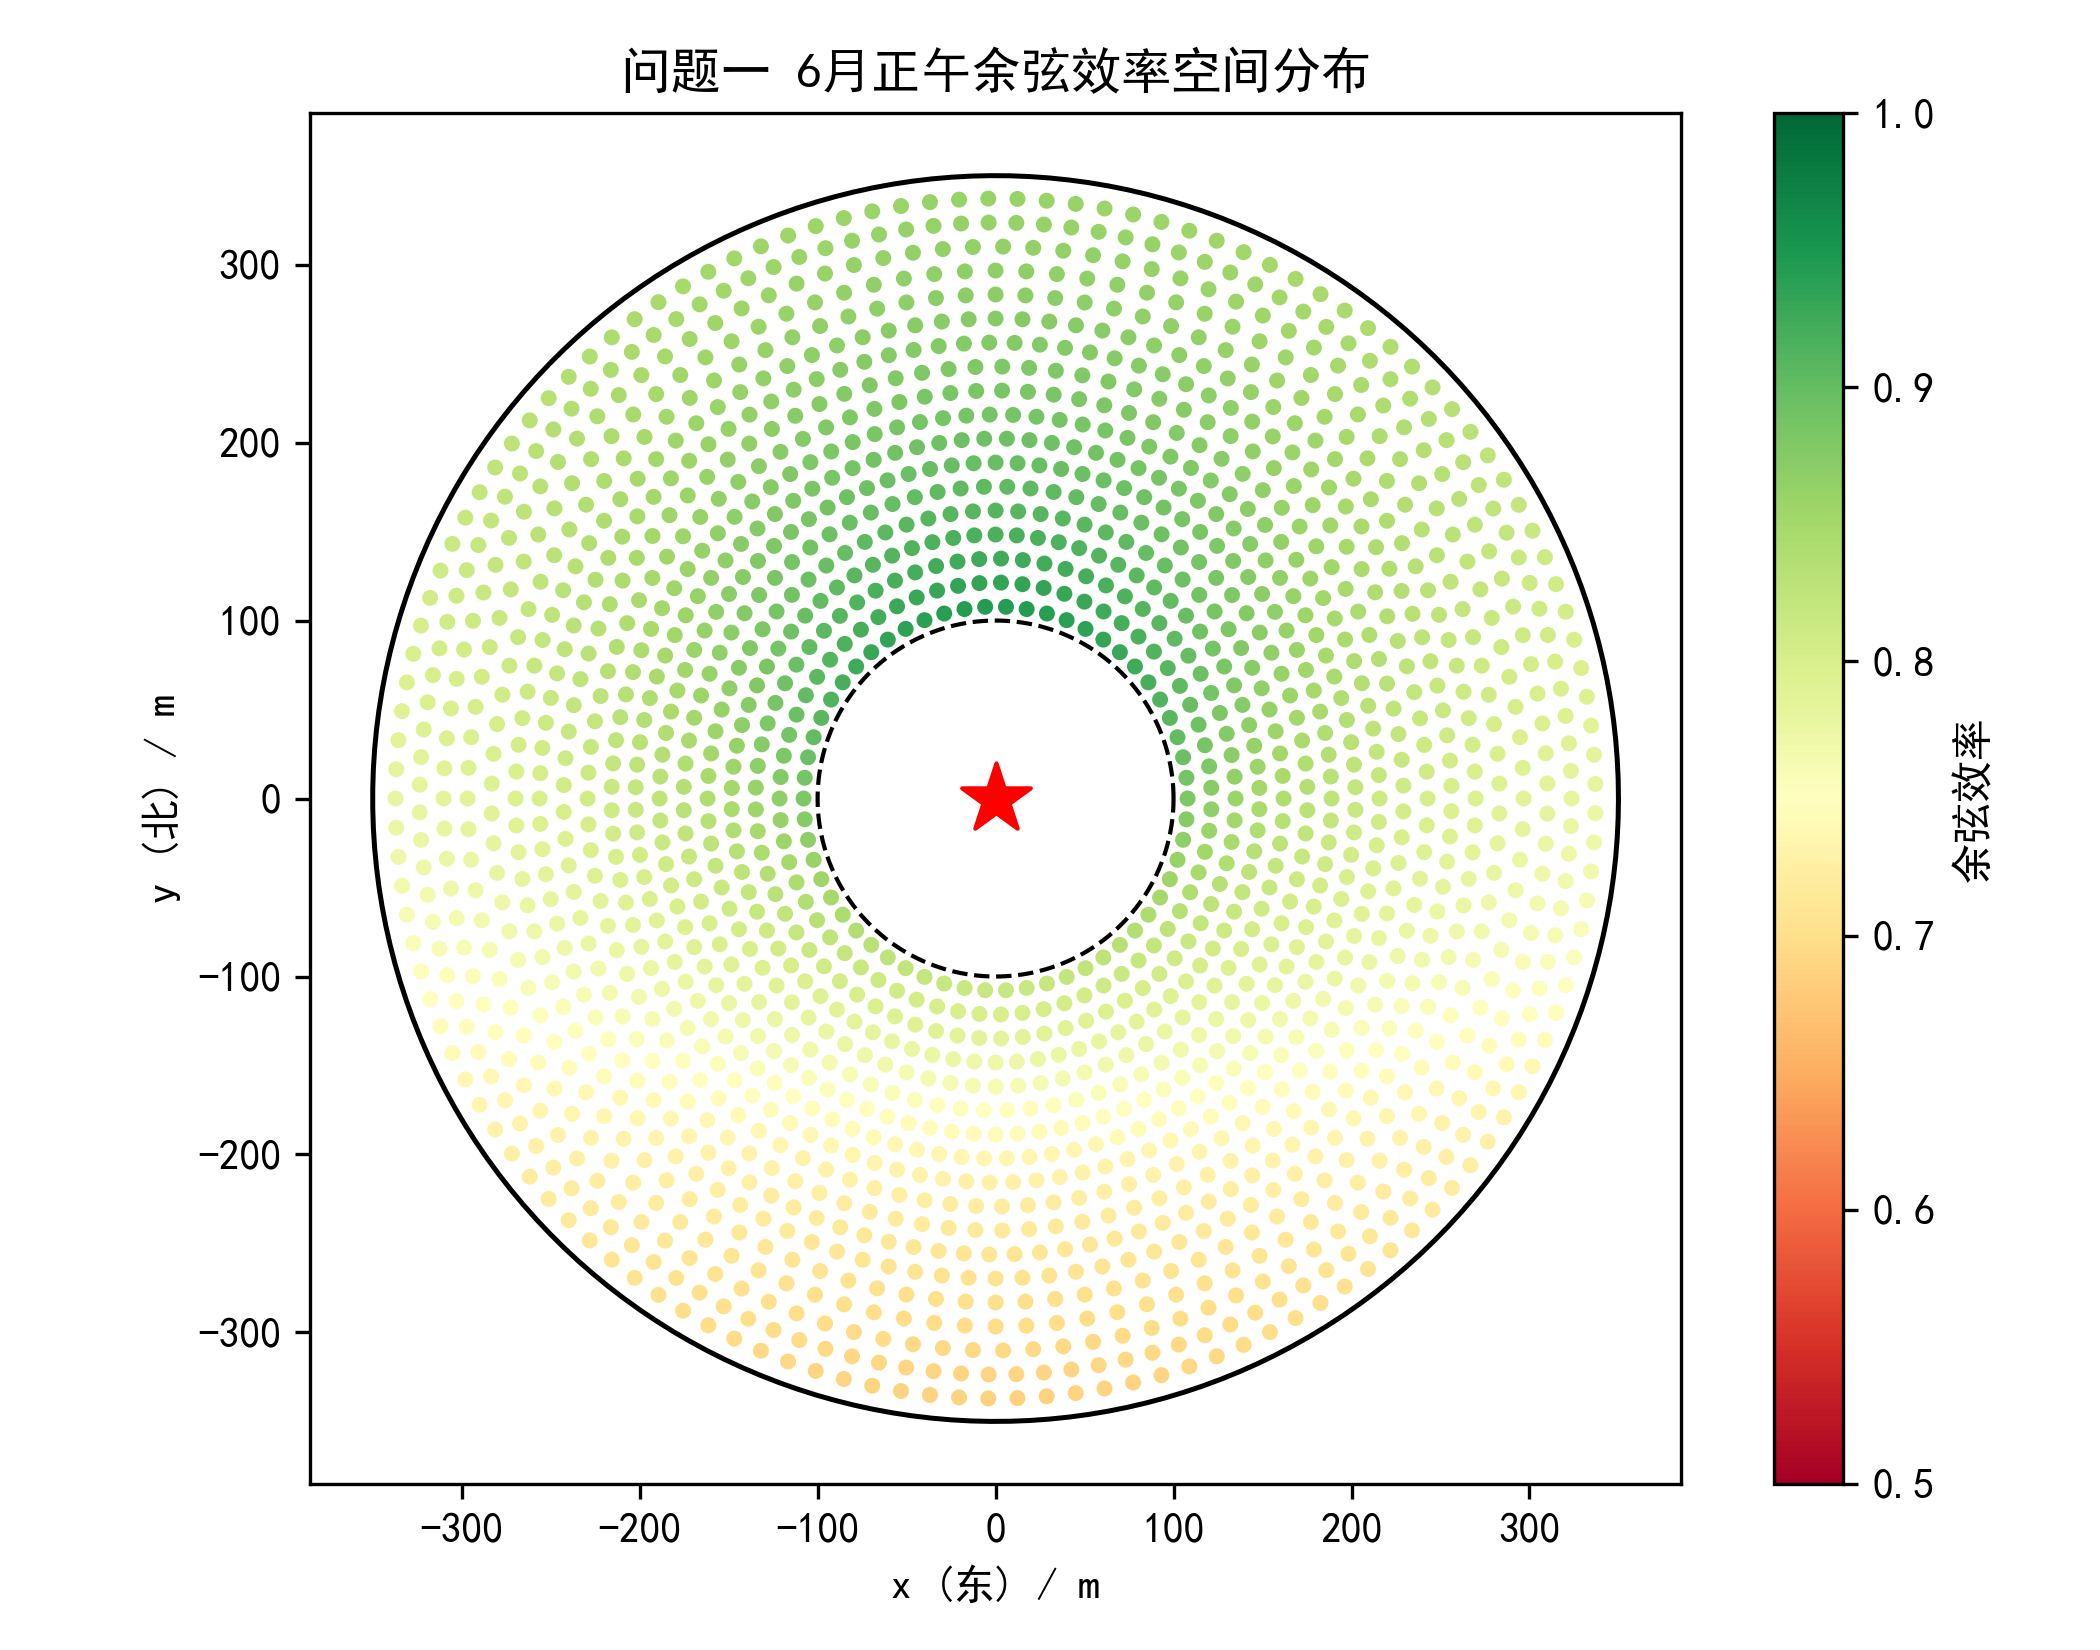
\includegraphics[width=0.7\textwidth]{fig8_cos_spatial.png}
\caption{问题一 $6$ 月正午余弦效率的空间分布}
\label{fig:fig8_cos_spatial}
\end{figure}

蒙特卡洛采样数 $K$ 的收敛性检验见表~\ref{tab:p1_conv}，$K=100$ 与 $K=300$ 的年平均效率差异小于 $0.01\%$，表明结果已收敛，$K=300$ 的统计误差可忽略。

\begin{table}[H]
\centering
\begin{tabular}{lccc}
\toprule
采样数 $K$ & 年平均光学效率 & 年平均输出热功率 (MW) \\
\midrule
100 & 0.60671 & 37.082 \\
300 & 0.60674 & 37.084 \\
\bottomrule
\end{tabular}
\caption{蒙特卡洛采样数收敛性检验}
\label{tab:p1_conv}
\end{table}

\section{问题二的求解}
\label{sec:p2}
\subsection{布局参数化与优化模型}
采用径向交错（radial stagger）布局：以吸收塔为圆心生成同心圆环，第 $k$ 环半径 $r_k=r_0+k\,d_r$，环向角间距为 $d_s$，相邻环错开半个角间距。为满足相邻底座中心距离大于镜面宽度加 $5$ m 的约束，采用六角密排 $d_r=\frac{\sqrt{3}}{2}d_s$，此时相邻定日镜间距恒为 $d_s$，故要求 $d_s>W+5$。布局以场地圆心（原点）为中心生成，吸收塔位置 $(x_t,y_t)$ 作为独立决策变量，吸收塔周围 $100$ m 内的镜子被剔除。

决策变量为 $\mathbf{x}=(x_t,y_t,W,H,h,r_0,d_s)$，优化模型为
\begin{equation}
\begin{aligned}
\max_{\mathbf{x}}\quad & \frac{E_{field}}{\sum_i A_i} \\
\text{s.t.}\quad & E_{field}\ge 60\ \text{MW},\quad W\ge H,\quad h\ge H/2,\\
& 2\le W,H\le 8,\quad 2\le h\le 6,\quad d_s>W+5.
\end{aligned}
\end{equation}

\subsection{阴影遮挡效率的标定}
优化需频繁评估目标函数，完整光线追踪计算量较大。为此，本文先通过完整光线追踪对径向交错布局的阴影遮挡效率进行标定，结果见表~\ref{tab:sb_calib}。标定中取 $d_s=11,13,16,20$ m（$W=6$ m），其中 $d_s=11$ m 对应最小间距 $W+5$ 的临界情形；实际优化中取 $d_s=W+5.05$ m，留出 $0.05$ m 裕量以严格满足"相邻底座中心距离比镜面宽度多 $5$ m 以上"的约束。随占空比 $W/d_s$ 增大（布局加密），阴影遮挡效率单调下降，拟合得到经验模型
\begin{equation}
\eta_{sb}=1-2.02\left(\frac{W}{d_s}\right)^{3.68},
\end{equation}
该模型在 $W/d_s\in[0.3,0.55]$ 范围内与完整光线追踪的误差小于 $2\%$。需要指出的是，该模型基于吸收塔位于圆心的对称布局标定，在吸收塔大幅偏移的非对称布局下偏差较大（例如塔向南偏移 $198$ m 时偏差约 $10\%$），会导致代理模型高估塔偏移的收益。为此，本文采用"代理模型粗搜 + 完整光线追踪精修"的两阶段策略：先用代理模型（余弦与大气透射解析计算、截断少量采样蒙特卡洛、阴影遮挡用上式）快速缩小搜索范围，再对候选解用完整光线追踪精确验证与微调，最终确定最优方案。这一策略避免了代理偏差导致的错误最优。

\begin{table}[H]
\centering
\begin{tabular}{lccccc}
\toprule
环向间距 $d_s$ (m) & 11 & 13 & 16 & 20 \\
\midrule
阴影遮挡效率 $\eta_{sb}$ & 0.784 & 0.865 & 0.932 & 0.976 \\
\bottomrule
\end{tabular}
\caption{阴影遮挡效率随间距的标定（$W=6$ m）}
\label{tab:sb_calib}
\end{table}

\subsection{吸收塔位置的关键作用}
当地太阳常年偏南，塔北侧的定日镜朝南反射、余弦效率高，塔南侧的定日镜需大角度偏转、余弦效率低。因此，将吸收塔向南偏移，使场地北侧留出更多空间布置高效定日镜，是提升整体效率的关键。固定布局、仅移动吸收塔的敏感性分析如图~\ref{fig:fig7_tower} 和表~\ref{tab:tower_sens} 所示：当塔由圆心向南偏移 $150$ m 时，余弦效率由 $0.754$ 提升至 $0.823$，单位面积功率由 $0.483$ 提升至 $0.518$ kW/m$^2$（代理模型，趋势与完整验证一致）。

\begin{figure}[H]
\centering
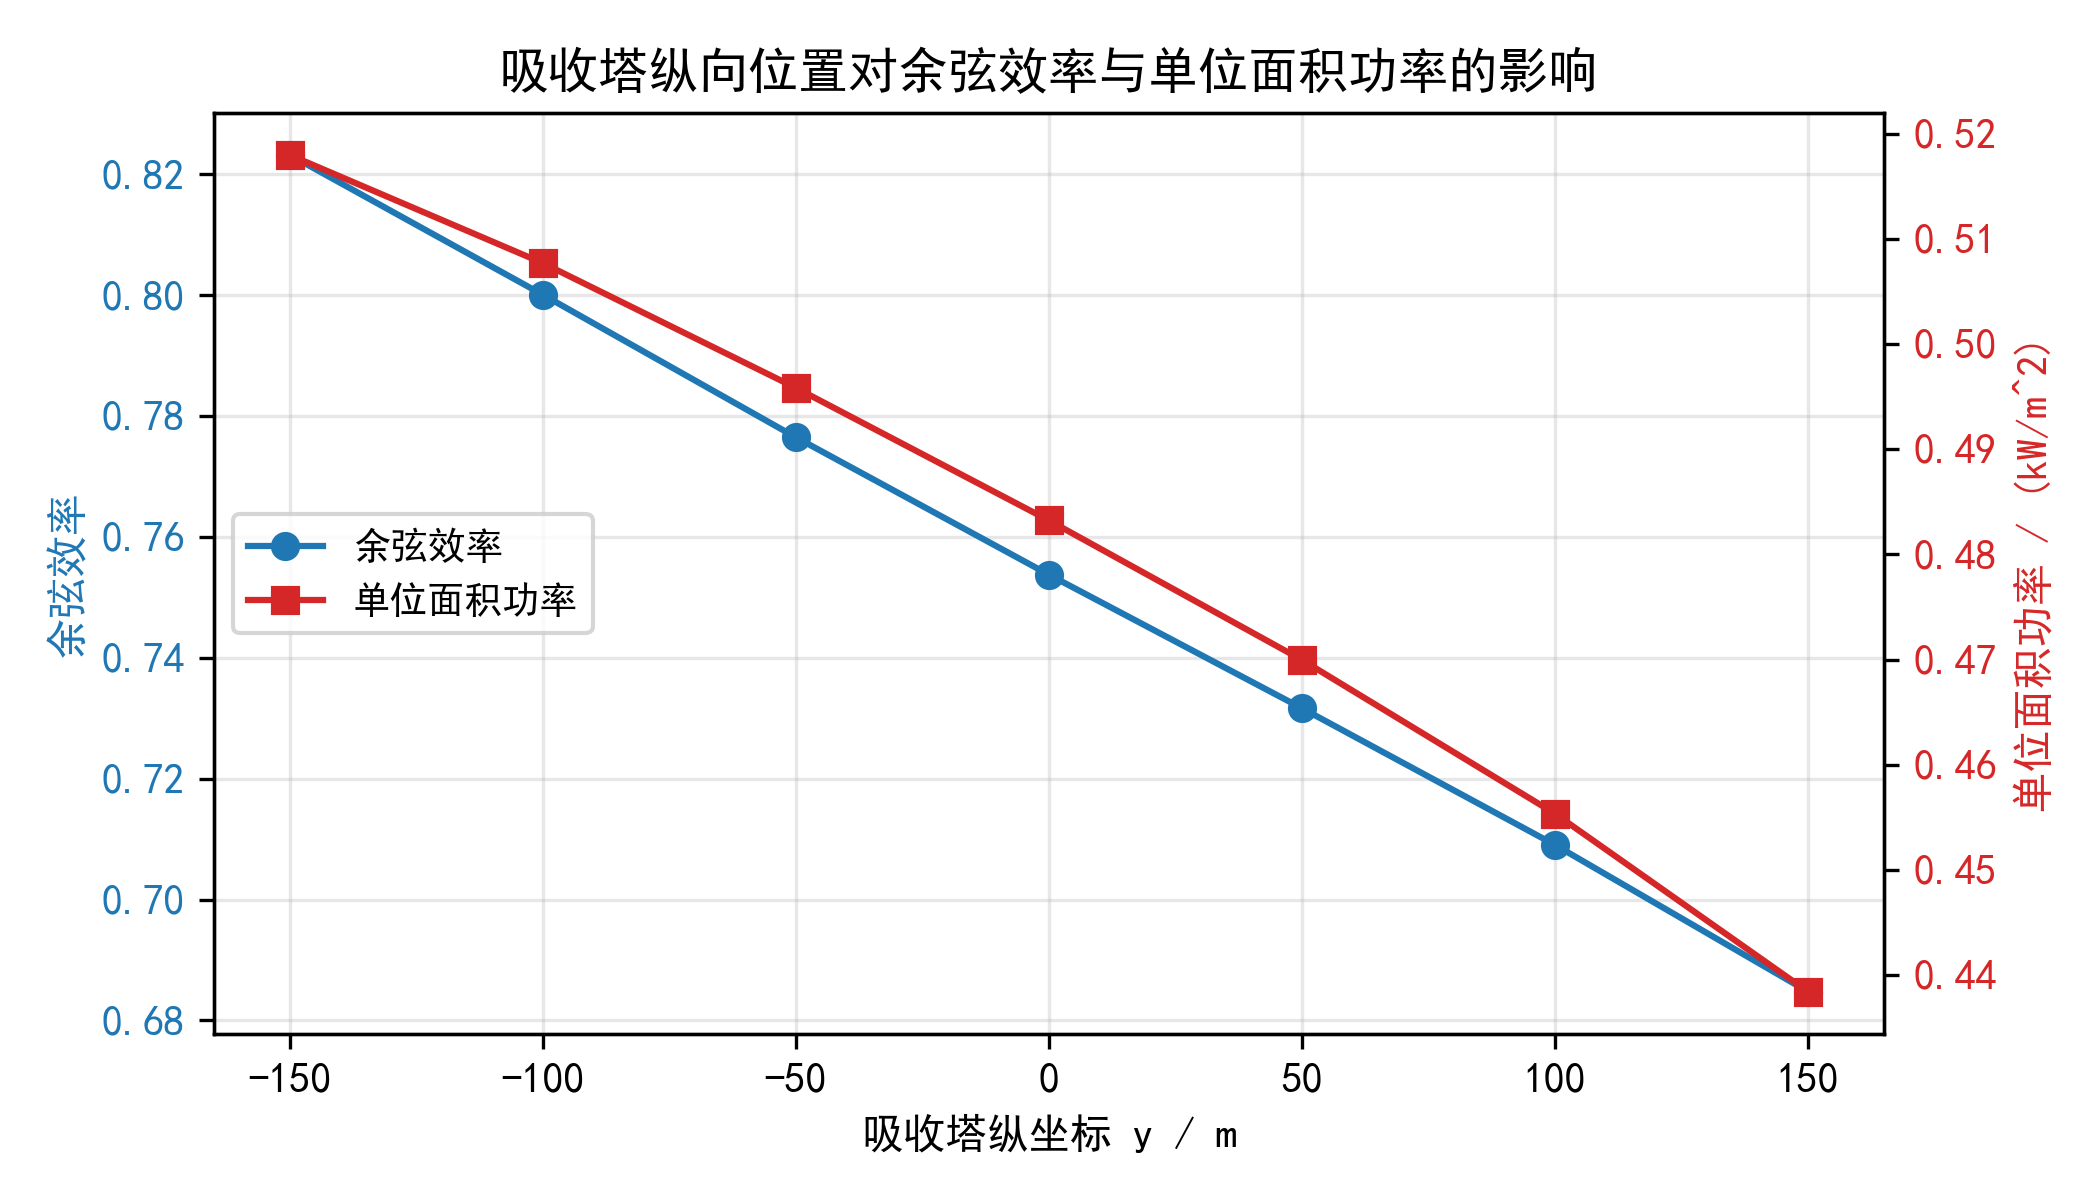
\includegraphics[width=0.75\textwidth]{fig7_tower.png}
\caption{吸收塔纵向位置对余弦效率与单位面积功率的影响}
\label{fig:fig7_tower}
\end{figure}

\begin{table}[H]
\centering
\resizebox{\textwidth}{!}{%
\begin{tabular}{lccccccc}
\toprule
塔纵坐标 $y_t$ (m) & $-150$ & $-100$ & $-50$ & $0$ & $50$ & $100$ & $150$ \\
\midrule
余弦效率 & 0.823 & 0.800 & 0.777 & 0.754 & 0.732 & 0.709 & 0.685 \\
单位面积功率 (kW/m$^2$) & 0.518 & 0.508 & 0.496 & 0.483 & 0.470 & 0.455 & 0.438 \\
\bottomrule
\end{tabular}%
}
\caption{吸收塔纵向位置的敏感性分析（固定布局）}
\label{tab:tower_sens}
\end{table}

\subsection{基准方案与优化方案对比}
为体现优化的有效性，本文采用双模型对比：\textbf{基准方案}为吸收塔位于圆心、定日镜 $6\times6$ m 的简单布置；\textbf{优化方案}为差分进化算法得到的方案。对比结果见表~\ref{tab:p2_compare}。基准方案尽管单位面积功率略高，但其输出热功率仅为 $54.7$ MW，未达到 $60$ MW 额定功率；若通过加密布局使其达标，单位面积功率将因阴影遮挡加剧而降至 $0.483$ kW/m$^2$。优化方案通过向南偏移吸收塔（余弦效率提升至 $0.816$），在满足额定功率的同时将单位面积功率提升至 $0.505$ kW/m$^2$，较塔位于圆心的达标方案提升 $4.6\%$。

\begin{table}[H]
\centering
\resizebox{\textwidth}{!}{%
\begin{tabular}{lcccccc}
\toprule
方案 & 塔位置 (m) & 定日镜尺寸 (m) & 面数 & 输出功率 (MW) & 单位面积功率 (kW/m$^2$) & 达标 \\
\midrule
基准（塔圆心） & $(0,0)$ & $6.0\times6.0$ & 2965 & 54.72 & 0.513 & 否 \\
塔圆心加密达标 & $(0,0)$ & $6.3\times6.27$ & 3155 & 60.14 & 0.483 & 是 \\
优化方案 & $(0,-120)$ & $6.0\times5.97$ & 3321 & 60.06 & 0.505 & 是 \\
\bottomrule
\end{tabular}%
}
\caption{问题二基准方案与优化方案对比}
\label{tab:p2_compare}
\end{table}

\subsection{求解算法与复杂度}
采用差分进化（DE）算法求解上述 $7$ 维连续优化问题。DE 通过种群内的差分变异与交叉产生新个体，全局搜索能力强、无需梯度，适合本问题的黑箱目标函数。算法步骤为：\textbf{①初始化} 在决策变量范围内随机生成规模为 $NP$ 的种群；\textbf{②变异} 对每个个体 $\mathbf{x}_i$，随机选三个互异个体生成变异向量 $\mathbf{v}_i=\mathbf{x}_{r1}+F(\mathbf{x}_{r2}-\mathbf{x}_{r3})$；\textbf{③交叉} 变异向量与父代逐维交叉生成试验向量；\textbf{④选择} 若试验向量目标更优则替换父代。算法设置缩放因子 $F=0.8$、交叉概率 $CR=0.9$，采用"先大种群粗搜、后局部搜索精修"的策略：以种群规模 $NP=30$、迭代 $60$ 次进行全局搜索（约 $1830$ 次目标评估），再对最优解用 L-BFGS-B 进行局部精细搜索。为验证收敛性，本文对比了 $NP=10$ 与 $NP=30$ 两种种群设置，二者经完整光线追踪验证的最优解一致（均为吸收塔向南偏移 $120$ m 附近），表明搜索已充分收敛。布局参数化将数千面镜子的坐标压缩为 $7$ 个参数，使目标函数可快速评估；单次代理评估约 $0.2$--$0.5$ s，总优化时间约 $11$ min。若定日镜数目进一步增长，可采用逐环并行评估或解析近似进一步提高效率，本方法的时间复杂度与镜子数目近乎线性，具有良好的可扩展性。

DE 算法的收敛过程如图~\ref{fig:fig11_de_convergence} 所示（纵轴为代理模型的单位面积功率）。算法在初始随机种群（单位面积功率仅 $0.181$ kW/m$^2$）基础上，前 $10$ 次迭代快速收敛至 $0.55$ kW/m$^2$ 附近，随后 $10$--$30$ 次迭代缓慢逼近最优解 $0.577$ kW/m$^2$。收敛过程无震荡、无早熟停滞，表明 DE 算法对本问题的全局搜索能力良好。需说明的是，代理模型因阴影遮挡的标定偏差，其绝对值（$0.577$）略高于完整光线追踪结果（$0.505$），但收敛趋势与最优解位置一致，代理模型仅用于引导搜索方向，最终结果以完整光线追踪为准。

\begin{figure}[H]
\centering
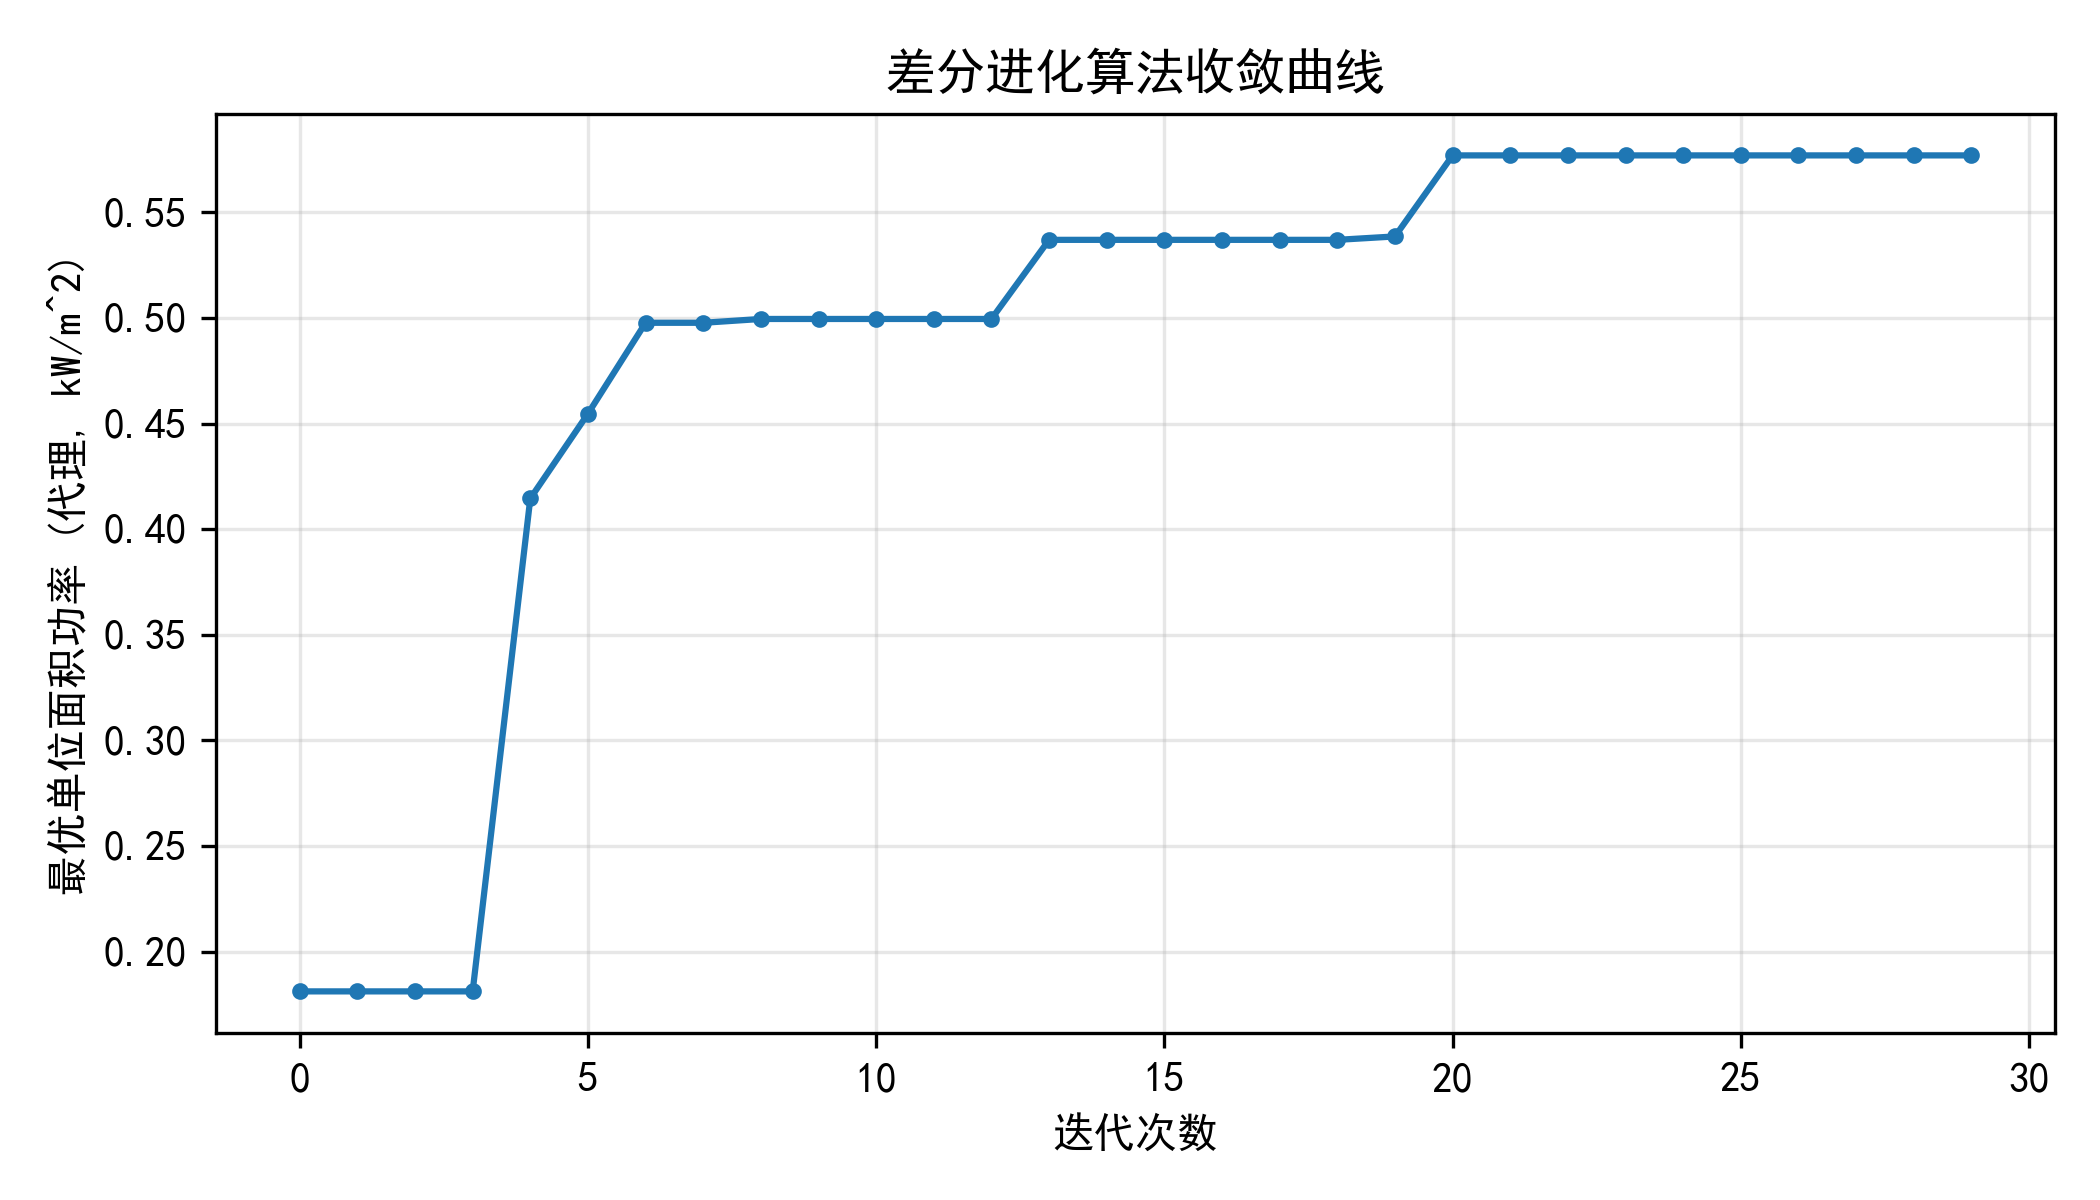
\includegraphics[width=0.75\textwidth]{fig11_de_convergence.png}
\caption{差分进化算法收敛曲线}
\label{fig:fig11_de_convergence}
\end{figure}

\subsection{定日镜尺寸的敏感性分析}
定日镜尺寸是影响单位面积功率的关键变量。固定吸收塔位置与布局间距，对定日镜宽度 $W$ 进行敏感性扫描（完整光线追踪），结果见表~\ref{tab:p2_Wsens}。随 $W$ 增大，定日镜光斑增大、截断效率下降，单位面积功率单调下降；同时镜面数与输出功率呈现非单调变化：$W$ 过小则镜面数虽多但面积不足，$W$ 过大则截断损失加剧。在额定功率 $60$ MW 约束下，$W=6.0$ m 是满足约束的最小尺寸，对应最高单位面积功率，因此优化方案选定 $W=6.0$ m。

\begin{table}[H]
\centering
\resizebox{\textwidth}{!}{%
\begin{tabular}{lccccc}
\toprule
定日镜宽度 $W$ (m) & 6.0 & 6.15 & 6.30 & 6.45 & 6.60 \\
\midrule
定日镜面数 & 3259 & 3240 & 3155 & 3009 & 2992 \\
截断效率 & 0.985 & 0.981 & 0.976 & 0.972 & 0.969 \\
年平均输出热功率 (MW) & 58.09 & 59.60 & 60.14 & 59.49 & 60.80 \\
单位面积功率 (kW/m$^2$) & 0.498 & 0.489 & 0.483 & 0.478 & 0.469 \\
\bottomrule
\end{tabular}%
}
\caption{定日镜宽度对输出功率与单位面积功率的影响（塔位于圆心）}
\label{tab:p2_Wsens}
\end{table}

布局间距 $d_s$ 通过两条途径影响结果：$d_s$ 减小使镜面数增加、总面积增大、输出功率增大，但同时使占空比 $W/d_s$ 增大、阴影遮挡加剧。由表~\ref{tab:sb_calib} 可知，$d_s$ 从 $20$ m 减至 $11$ m 时，阴影遮挡效率从 $0.976$ 降至 $0.784$。优化中，$d_s$ 取满足间距约束的最小值附近（$d_s\approx W+5$），以在阴影遮挡损失可接受的前提下最大化镜面数，从而满足 $60$ MW 额定功率。这一权衡体现了问题二"在额定功率约束下最大化效率"的实质：密排换取功率、稀疏换取效率，最优解恰在两者平衡处。

\subsection{优化结果}
最优方案的设计参数见表~\ref{tab:p2_param}，完整光线追踪验证的年平均效率见表~\ref{tab:p2_annual}，最优布局与逐月效率如图~\ref{fig:fig4_p2_layout}、图~\ref{fig:fig5_p2_monthly} 所示。

\begin{table}[H]
\centering
\resizebox{\textwidth}{!}{%
\begin{tabular}{lcccc}
\toprule
吸收塔位置坐标 (m) & 定日镜尺寸 (宽$\times$高, m) & 安装高度 (m) & 定日镜总面数 & 定日镜总面积 (m$^2$) \\
\midrule
$(0,-120)$ & $6.0\times5.97$ & $3.15$ & $3321$ & $119021$ \\
\bottomrule
\end{tabular}%
}
\caption{问题二设计参数表}
\label{tab:p2_param}
\end{table}

\begin{table}[H]
\centering
\resizebox{\textwidth}{!}{%
\begin{tabular}{lccccc}
\toprule
 & 年平均光学效率 & 年平均余弦效率 & 年平均阴影遮挡效率 & 年平均截断效率 & 单位面积年平均输出热功率 (kW/m$^2$) \\
\midrule
数值 & 0.519 & 0.816 & 0.753 & 0.970 & 0.505 \\
\bottomrule
\end{tabular}%
}
\caption{问题二年平均光学效率及输出功率表}
\label{tab:p2_annual}
\end{table}

最优方案的吸收塔位于 $(0,-120)$ m，向南偏移 $120$ m；定日镜尺寸 $6.0\times5.97$ m，共 $3321$ 面，总面积 $119021$ m$^2$；年平均输出热功率 $60.06$ MW，达到额定功率，单位镜面面积年平均输出热功率 $0.505$ kW/m$^2$。与问题一相比，余弦效率由 $0.756$ 提升至 $0.816$（吸收塔南移的贡献），但布局加密使阴影遮挡效率由 $0.929$ 降至 $0.753$，这是满足额定功率约束所付出的密度代价。

\begin{figure}[H]
\centering
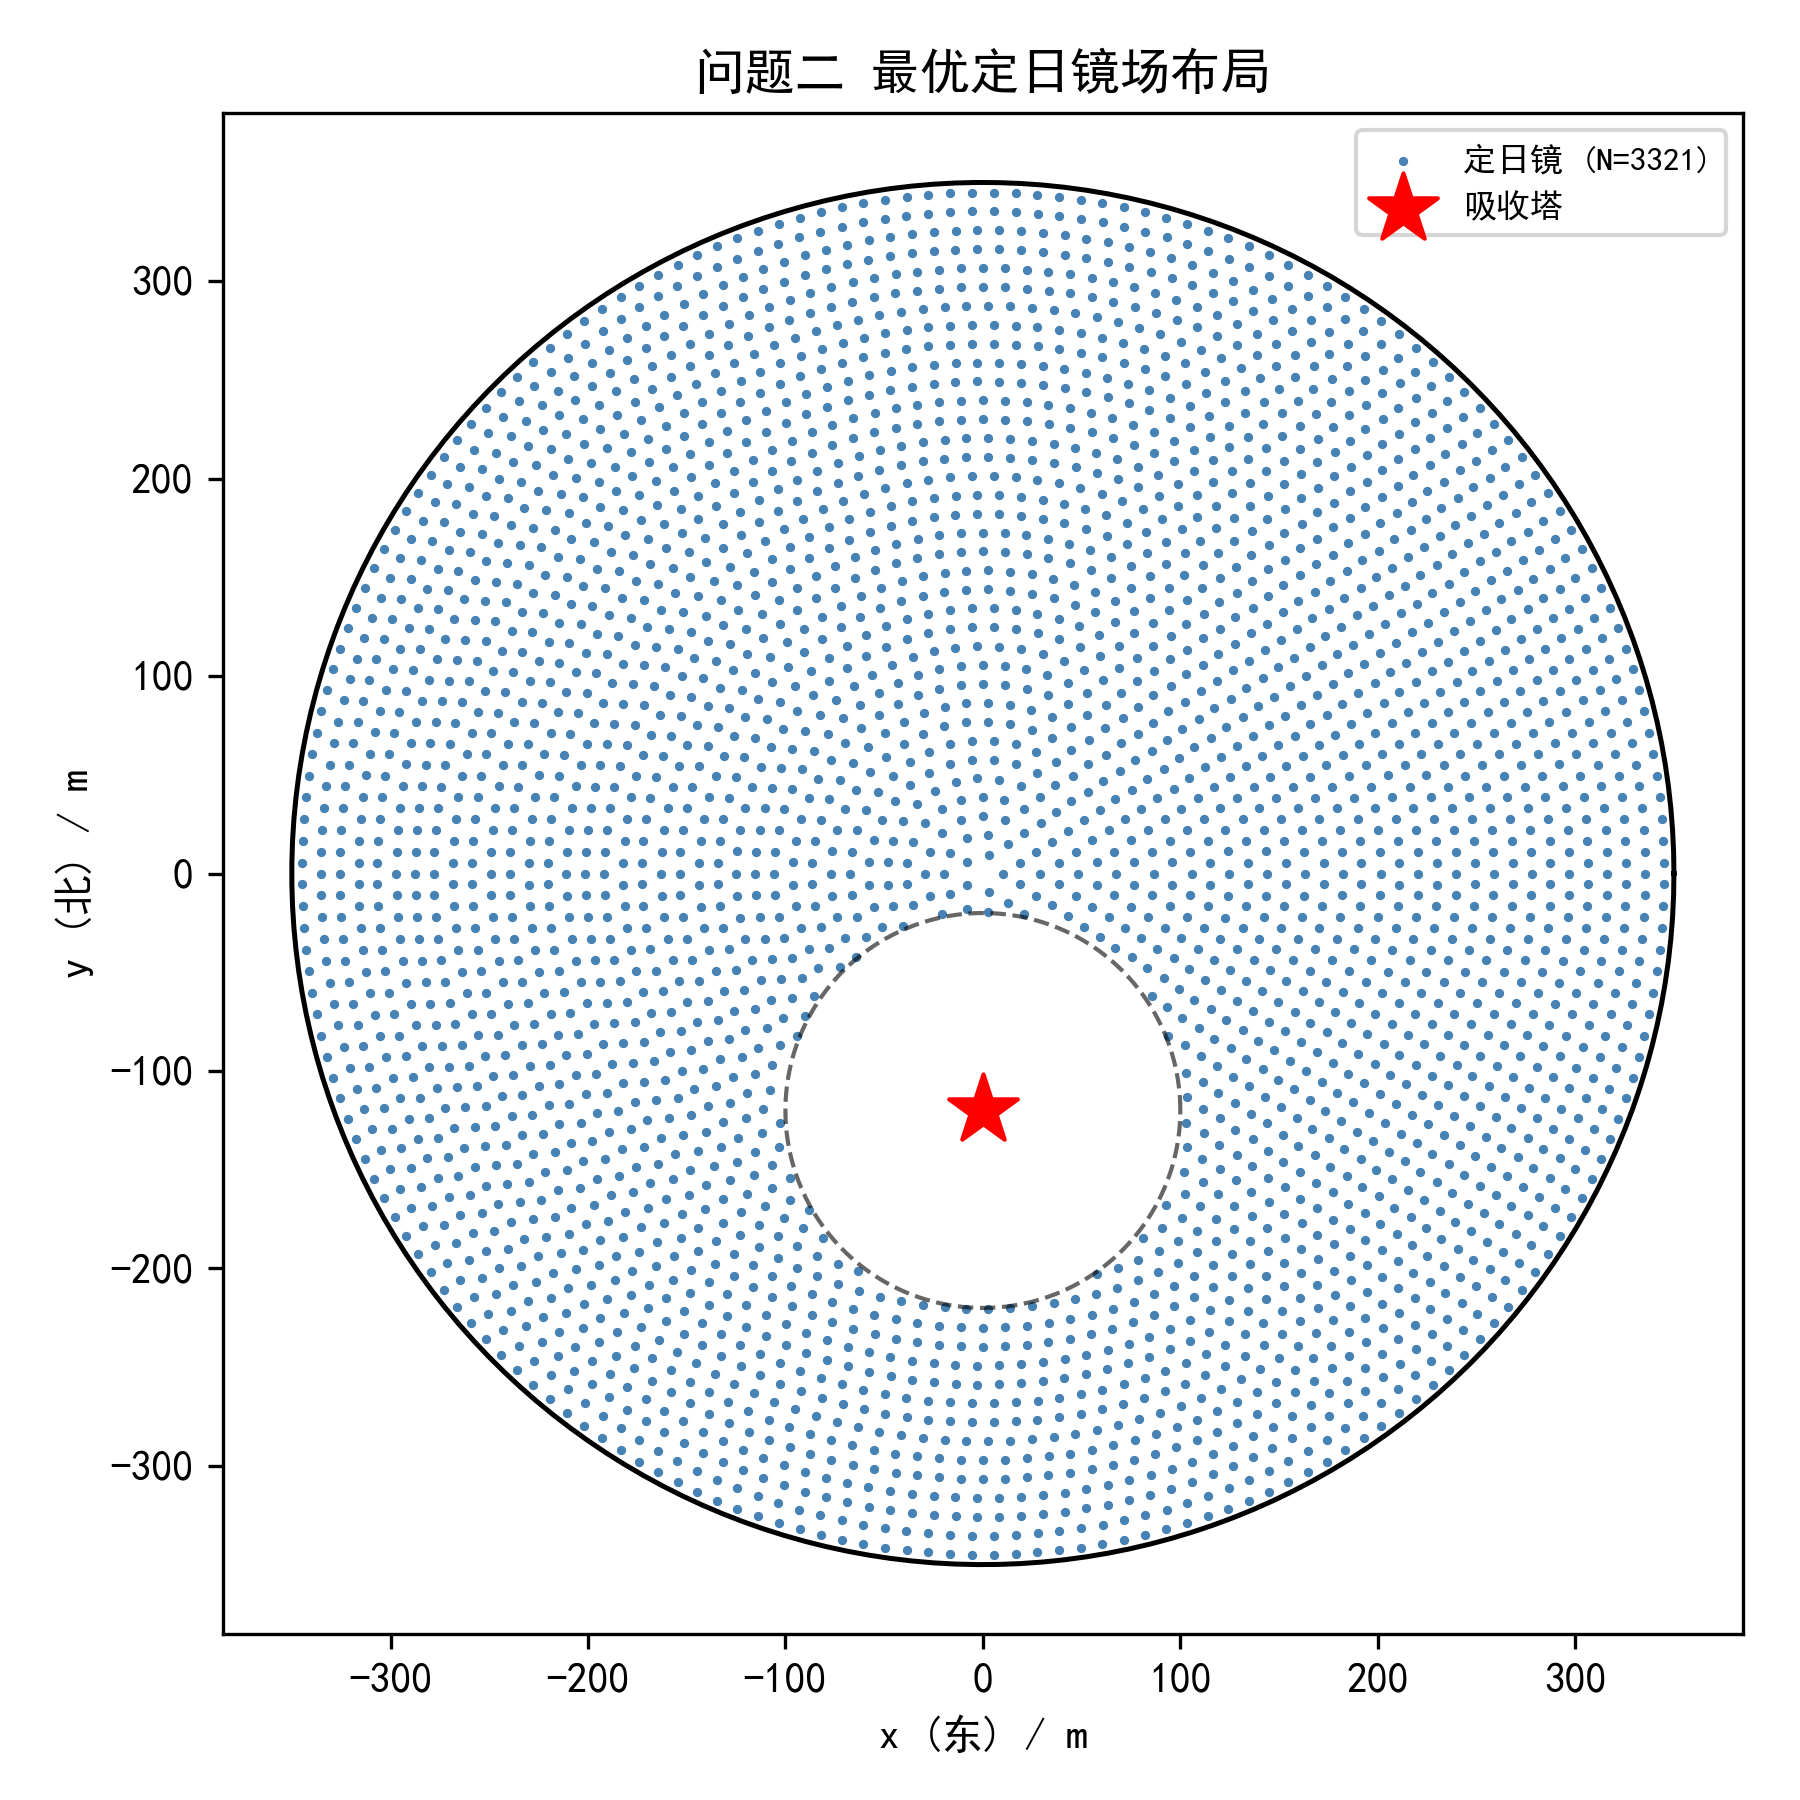
\includegraphics[width=0.62\textwidth]{fig4_p2_layout.png}
\caption{问题二最优定日镜场布局}
\label{fig:fig4_p2_layout}
\end{figure}

最优布局中，吸收塔南移后北侧空间更大，塔北侧（$y>-120$ m）的镜子数量占绝对多数；且北侧镜子的余弦效率（$0.851$）显著高于南侧（$0.782$），如图~\ref{fig:fig9_p2_cos_spatial} 所示。这一空间分布直观验证了吸收塔南移策略的有效性：将尽可能多的定日镜布置在高余弦效率的北侧区域，同时将南侧低效区域留给吸收塔及厂房。

\begin{figure}[H]
\centering
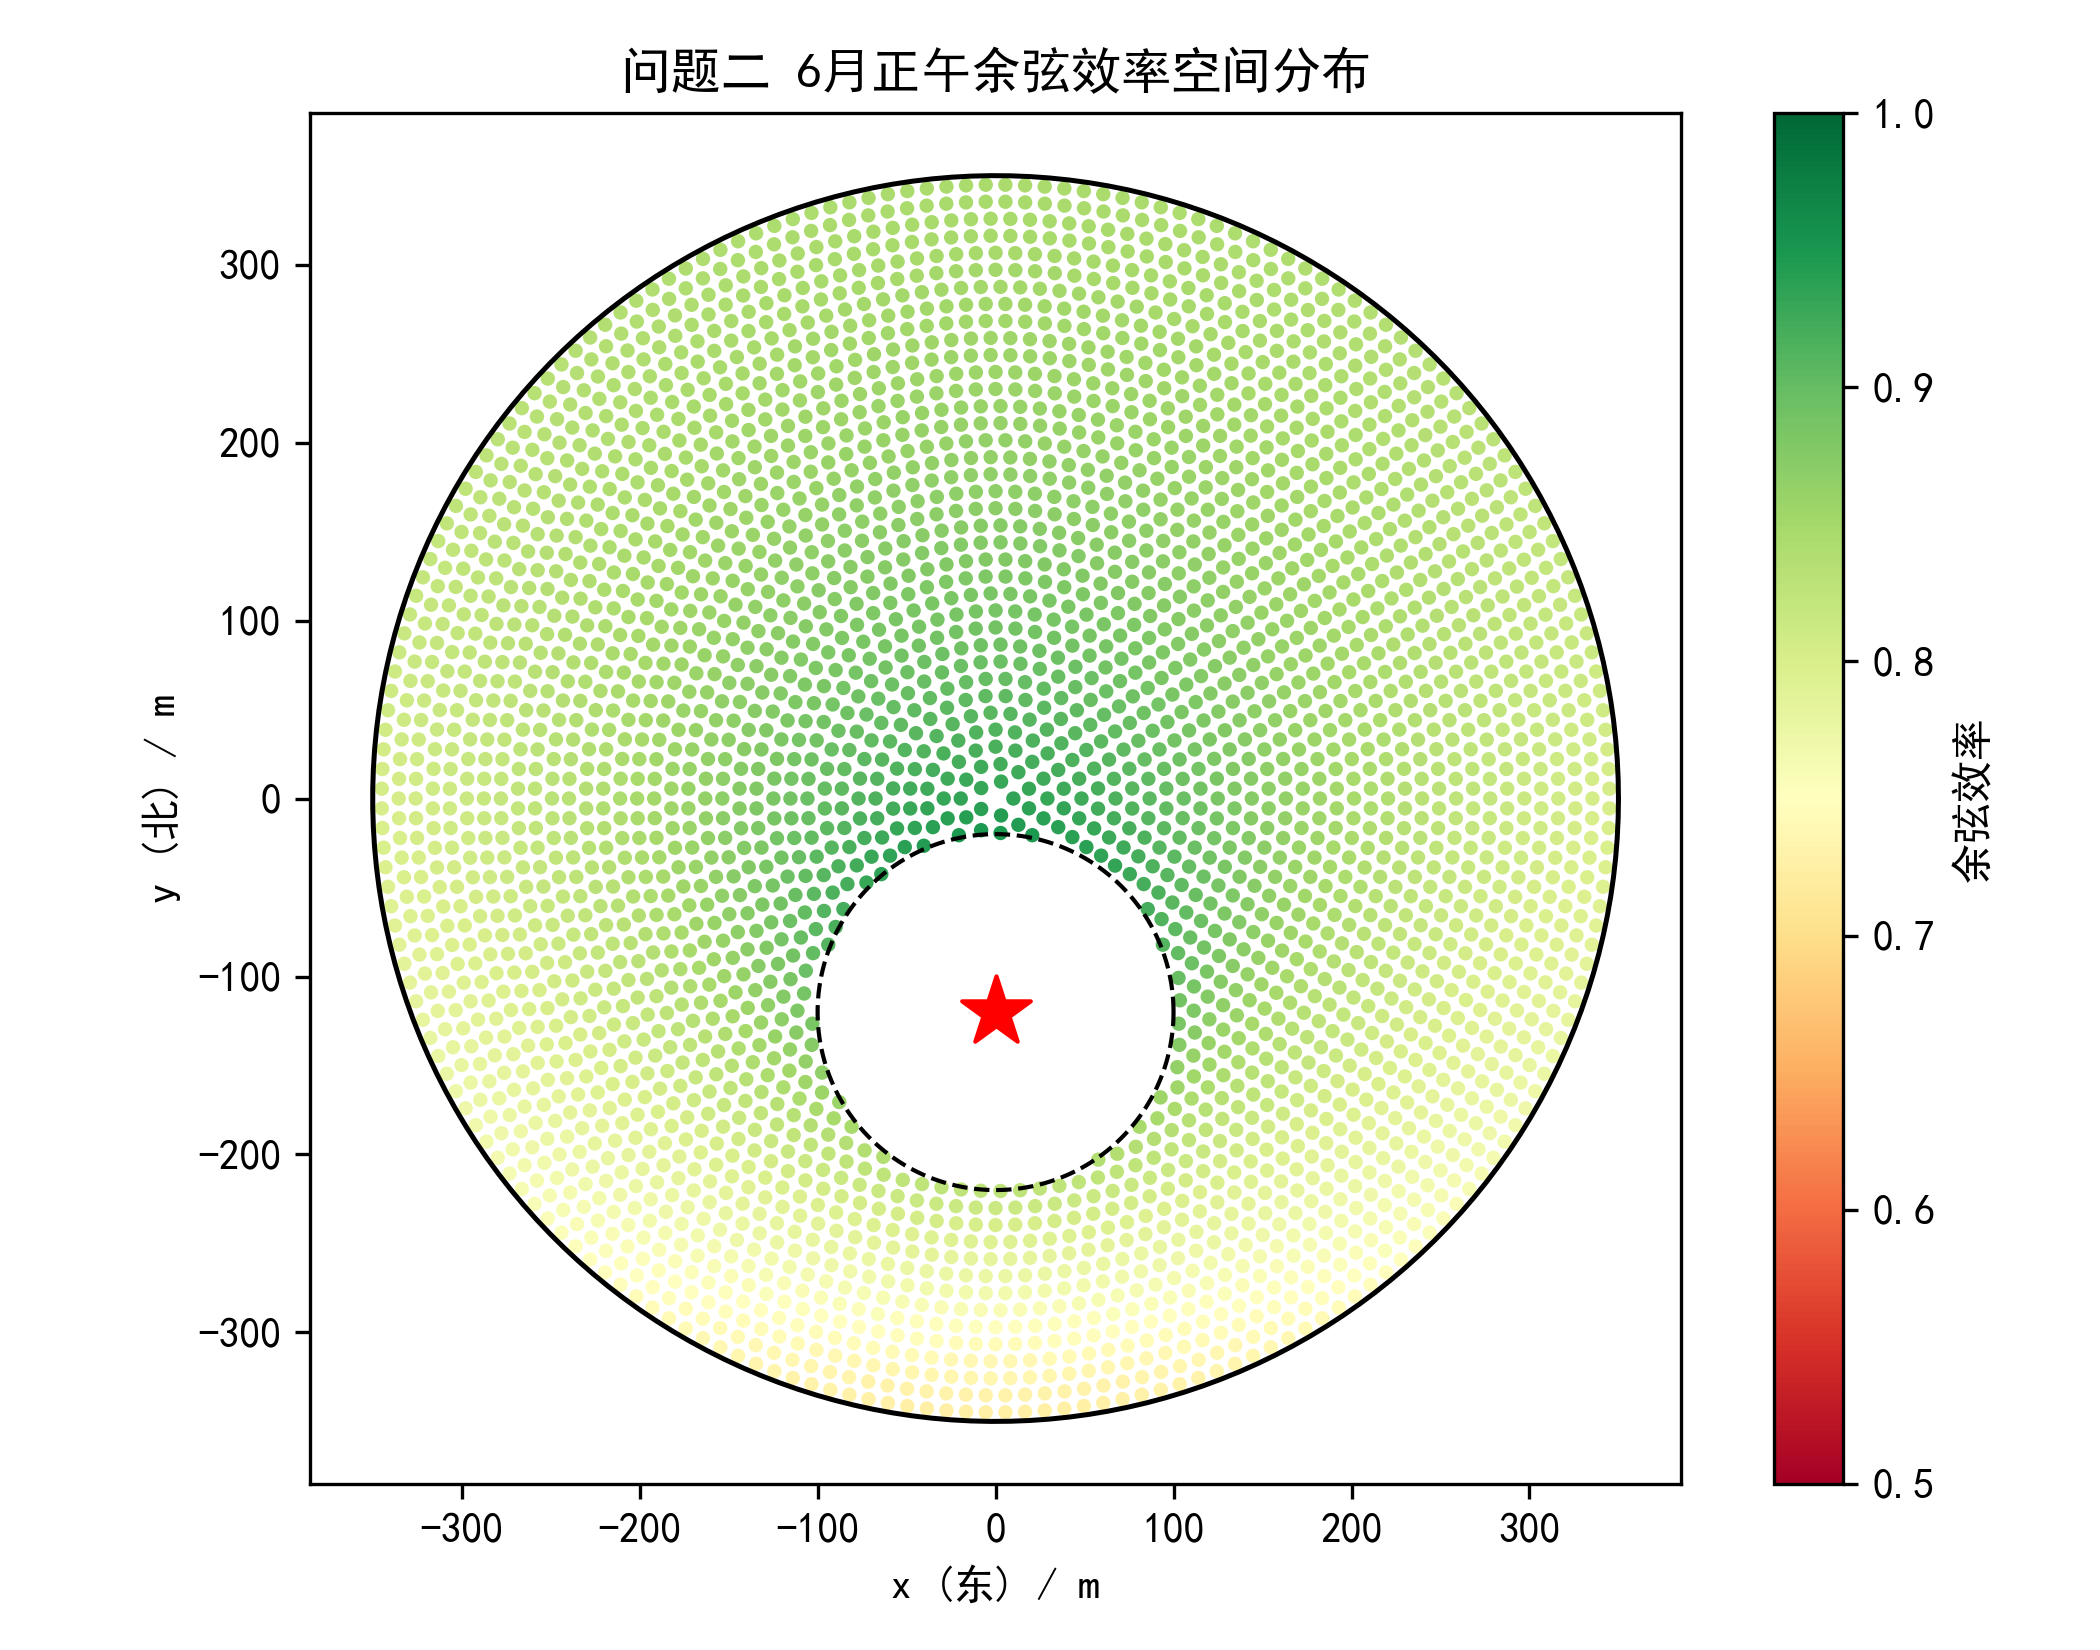
\includegraphics[width=0.7\textwidth]{fig9_p2_cos_spatial.png}
\caption{问题二 $6$ 月正午余弦效率的空间分布}
\label{fig:fig9_p2_cos_spatial}
\end{figure}

\begin{figure}[H]
\centering
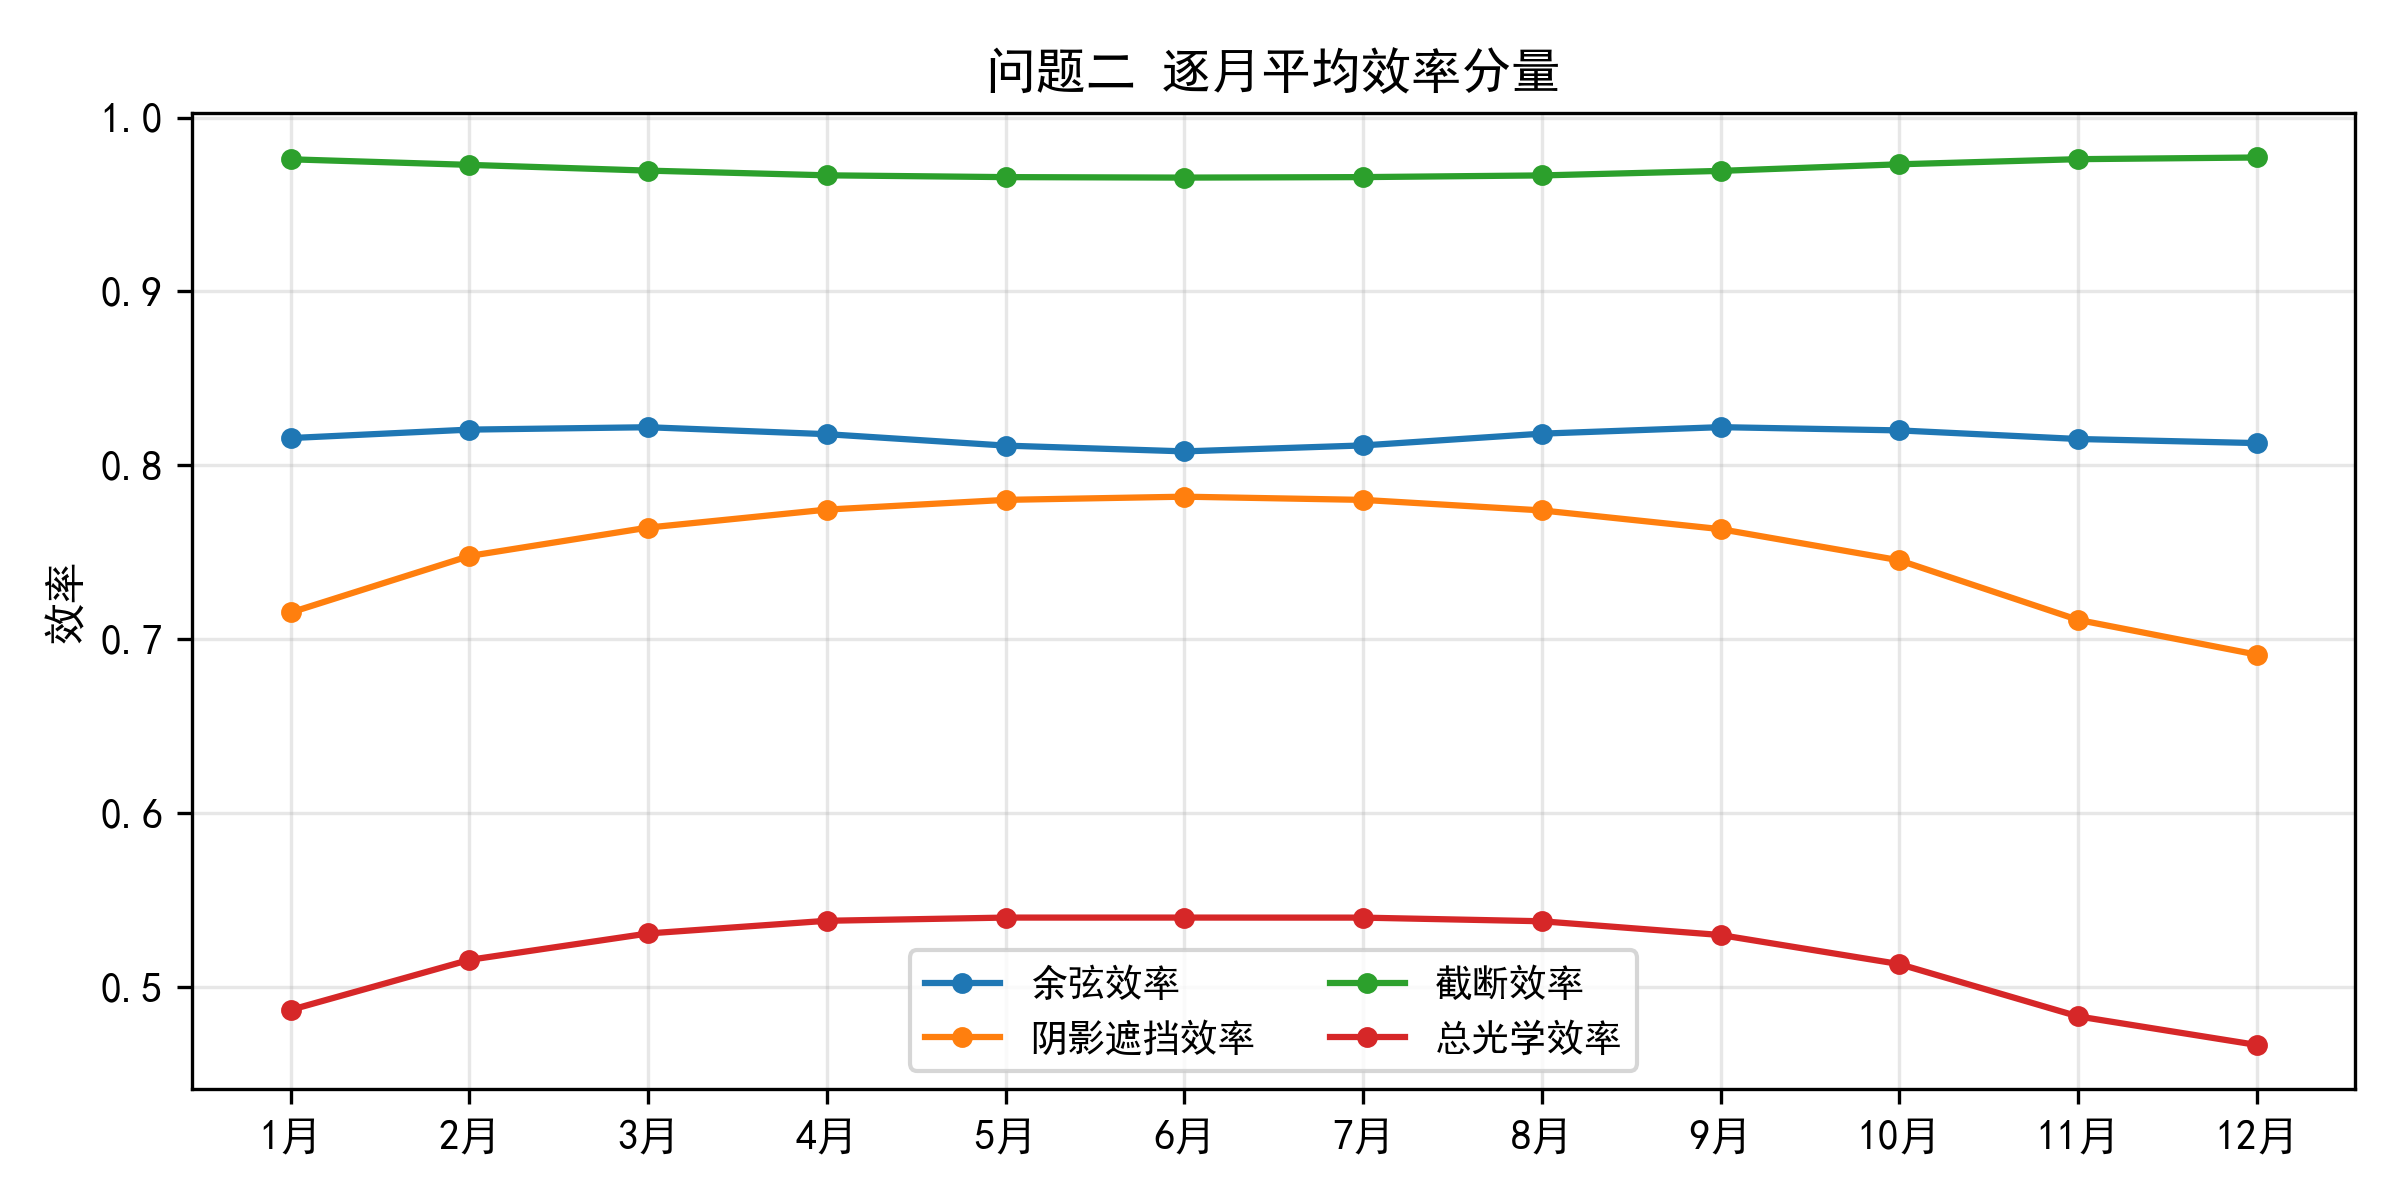
\includegraphics[width=0.85\textwidth]{fig5_p2_monthly.png}
\caption{问题二逐月平均效率分量}
\label{fig:fig5_p2_monthly}
\end{figure}

从逐月结果看，问题二的光学效率在 $6$ 月最高（$0.540$）、$12$ 月最低（$0.467$），季节变化幅度约 $0.073$，小于问题一的 $0.091$。值得注意的是，吸收塔南移后余弦效率的季节变化明显减小（问题二 $0.808$--$0.822$，问题一 $0.711$--$0.792$），这是因为北侧镜子朝南反射，全年的入射角都较小，受太阳高度角季节变化的影响减弱；而阴影遮挡效率仍呈现明显的冬低夏高（$0.691$--$0.782$），是效率季节波动的主要来源。逐月数据详见表~\ref{tab:p2_monthly}。

\begin{table}[H]
\centering
\resizebox{\textwidth}{!}{%
\begin{tabular}{lccccc}
\toprule
日期 & 平均光学效率 & 平均余弦效率 & 平均阴影遮挡效率 & 平均截断效率 & 单位面积平均输出热功率 (kW/m$^2$) \\
\midrule
 1月21日 & 0.487 & 0.816 & 0.716 & 0.976 & 0.426 \\
 2月21日 & 0.516 & 0.821 & 0.748 & 0.973 & 0.487 \\
 3月21日 & 0.531 & 0.822 & 0.764 & 0.969 & 0.528 \\
 4月21日 & 0.538 & 0.818 & 0.775 & 0.967 & 0.554 \\
 5月21日 & 0.540 & 0.811 & 0.780 & 0.966 & 0.564 \\
 6月21日 & 0.540 & 0.808 & 0.782 & 0.965 & 0.567 \\
 7月21日 & 0.540 & 0.812 & 0.780 & 0.966 & 0.564 \\
 8月21日 & 0.538 & 0.818 & 0.774 & 0.967 & 0.553 \\
 9月21日 & 0.530 & 0.822 & 0.763 & 0.969 & 0.526 \\
10月21日 & 0.513 & 0.820 & 0.746 & 0.973 & 0.481 \\
11月21日 & 0.483 & 0.815 & 0.711 & 0.976 & 0.419 \\
12月21日 & 0.467 & 0.813 & 0.691 & 0.977 & 0.390 \\
\bottomrule
\end{tabular}%
}
\caption{问题二每月 $21$ 日平均光学效率及输出功率}
\label{tab:p2_monthly}
\end{table}

结果的方向一致性可逐一验证：\textbf{①吸收塔南移}使余弦效率由 $0.756$ 升至 $0.816$（提升 $7.9\%$），机制是北侧镜子朝南反射、入射角减小；\textbf{②布局加密}（面数由 $1745$ 增至 $3321$）使阴影遮挡效率由 $0.929$ 降至 $0.753$（下降 $18.9\%$），机制是占空比增大、镜子间相互遮挡加剧；\textbf{③定日镜尺寸增大}（由 $6.0$ m 增至 $6.6$ m）使截断效率由 $0.985$ 降至 $0.969$，机制是光斑增大、溢出集热器。各项因素的符号与量级均符合物理预期，无反常或矛盾结果，验证了模型的正确性。

问题一与问题二的逐月输出热功率对比如图~\ref{fig:fig12_power_compare} 所示。问题二的输出热功率在冬季最低（$12$ 月 $44.7$ MW）、夏季最高（$6$ 月 $69.3$ MW），全年仅 $12$ 月、$1$ 月、$11$ 月低于额定功率 $60$ MW，其余月份均达标，年平均 $60.06$ MW 恰好满足约束；问题一的输出热功率全年仅 $28.8$--$42.3$ MW，远低于额定功率。问题二相对问题一的功率提升来自两方面：一是吸收塔南移使余弦效率提升 $7.9\%$，二是布局加密使镜面数由 $1745$ 增至 $3321$ 面（面积增大 $89\%$）。

\begin{figure}[H]
\centering
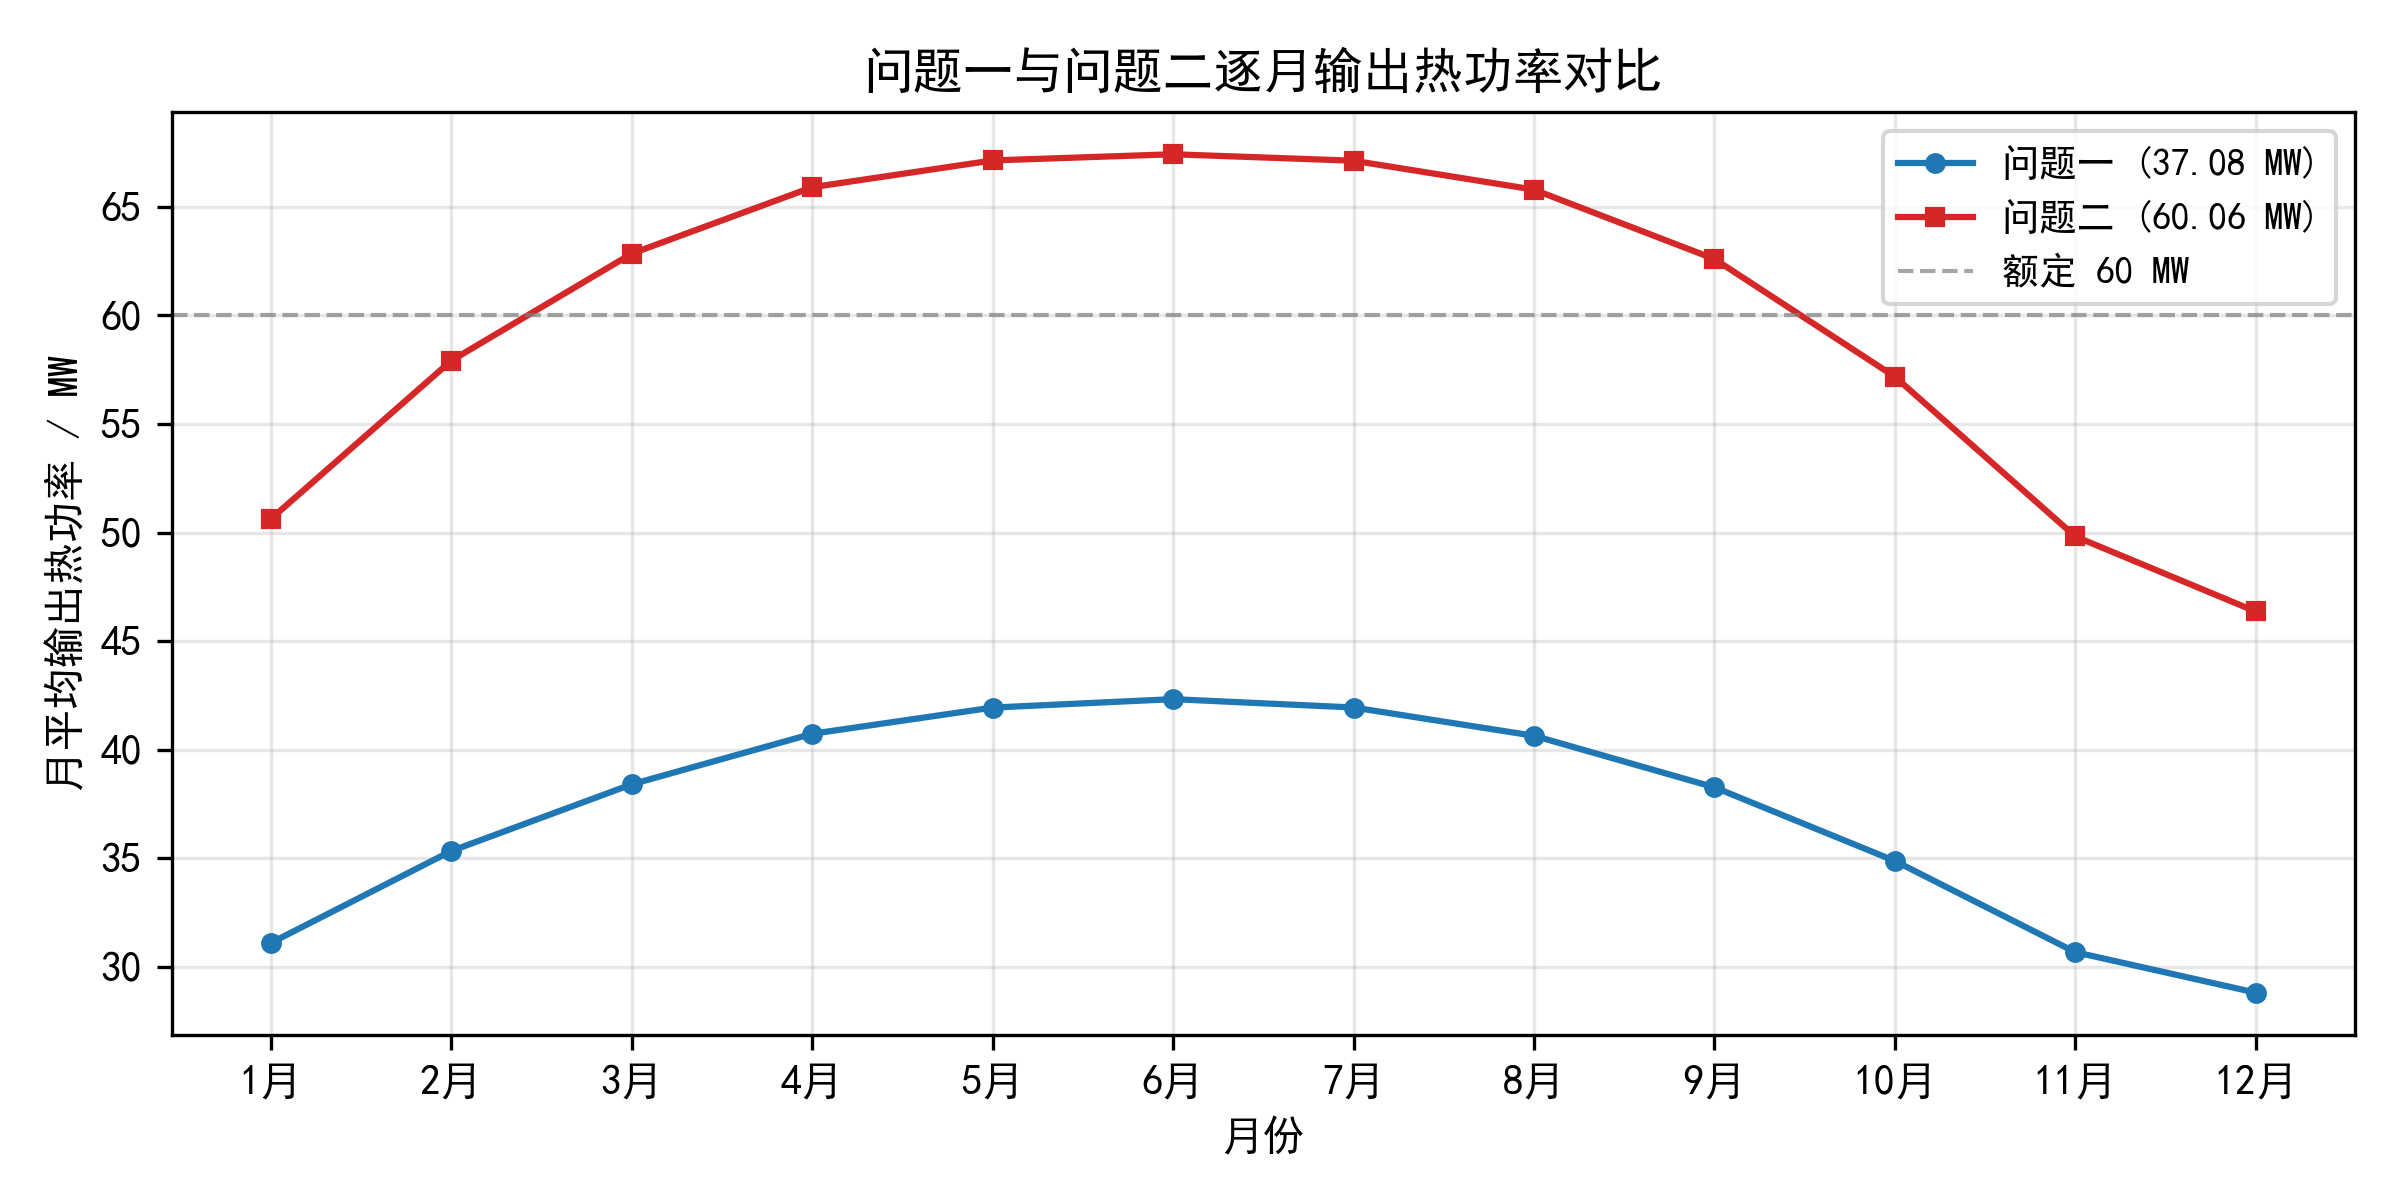
\includegraphics[width=0.85\textwidth]{fig12_power_compare.png}
\caption{问题一与问题二逐月输出热功率对比}
\label{fig:fig12_power_compare}
\end{figure}

\section{问题三的求解}
\label{sec:p3}
在问题二基础上，允许定日镜尺寸与安装高度随径向距离变化。由截断效率的物理机理可知，光斑尺寸约等于镜面投影加太阳锥扩散 $d\cdot\tan(4.65\times10^{-3})$，镜面尺寸越大、光斑越接近集热器直径（$7$ m），截断损失越大；而外环定日镜距离远、锥扩散大，宜采用较小尺寸以减小光斑。

本文采用尺寸随环半径线性变化的策略，引入内环与外环两组尺寸参数，并允许每环独立间距（外环小镜子采用更小间距以充分利用场地），沿用径向交错布局与 DE 算法求解。结果表明，内大外小的差异化尺寸可进一步提升单位面积功率：外环小镜子减小了光斑、提高了截断效率（由 $0.970$ 提升至 $0.975$），使单位面积功率由 $0.505$ 提升至 $0.512$ kW/m$^2$，较问题二提升 $1.4\%$（见表~\ref{tab:p3_compare}）。最优方案为内环 $6.6$ m、外环 $5.5$ m 线性过渡，共 $3455$ 面，年平均输出热功率 $60.00$ MW。

\begin{table}[H]
\centering
\resizebox{\textwidth}{!}{%
\begin{tabular}{lccc}
\toprule
尺寸方案 & 面数 & 输出功率 (MW) & 单位面积功率 (kW/m$^2$) \\
\midrule
均匀 $6.0$（问题二） & 3321 & 60.06 & 0.505 \\
内大外小 $6.5/5.5$ & 3436 & 59.39 & 0.515 \\
内大外小 $6.6/5.5$（最优） & 3455 & 60.00 & 0.512 \\
\bottomrule
\end{tabular}%
}
\caption{问题三尺寸方案对比（完整光线追踪）}
\label{tab:p3_compare}
\end{table}

最优方案的尺寸分布如图~\ref{fig:fig10_p3_size} 所示，定日镜宽度随径向距离线性减小，由内环的 $6.6$ m 过渡到外环的 $5.5$ m。这一设计的内在逻辑是：外环定日镜到集热器的距离大、太阳锥扩散大，采用小镜子可减小光斑、抑制截断损失；内环定日镜距离近，可采用较大镜子以提高单位镜面面积利用率。内外环的差异化使外环截断效率提升约 $0.005$，从而带来整体单位面积功率 $1.4\%$ 的提升。

\begin{figure}[H]
\centering
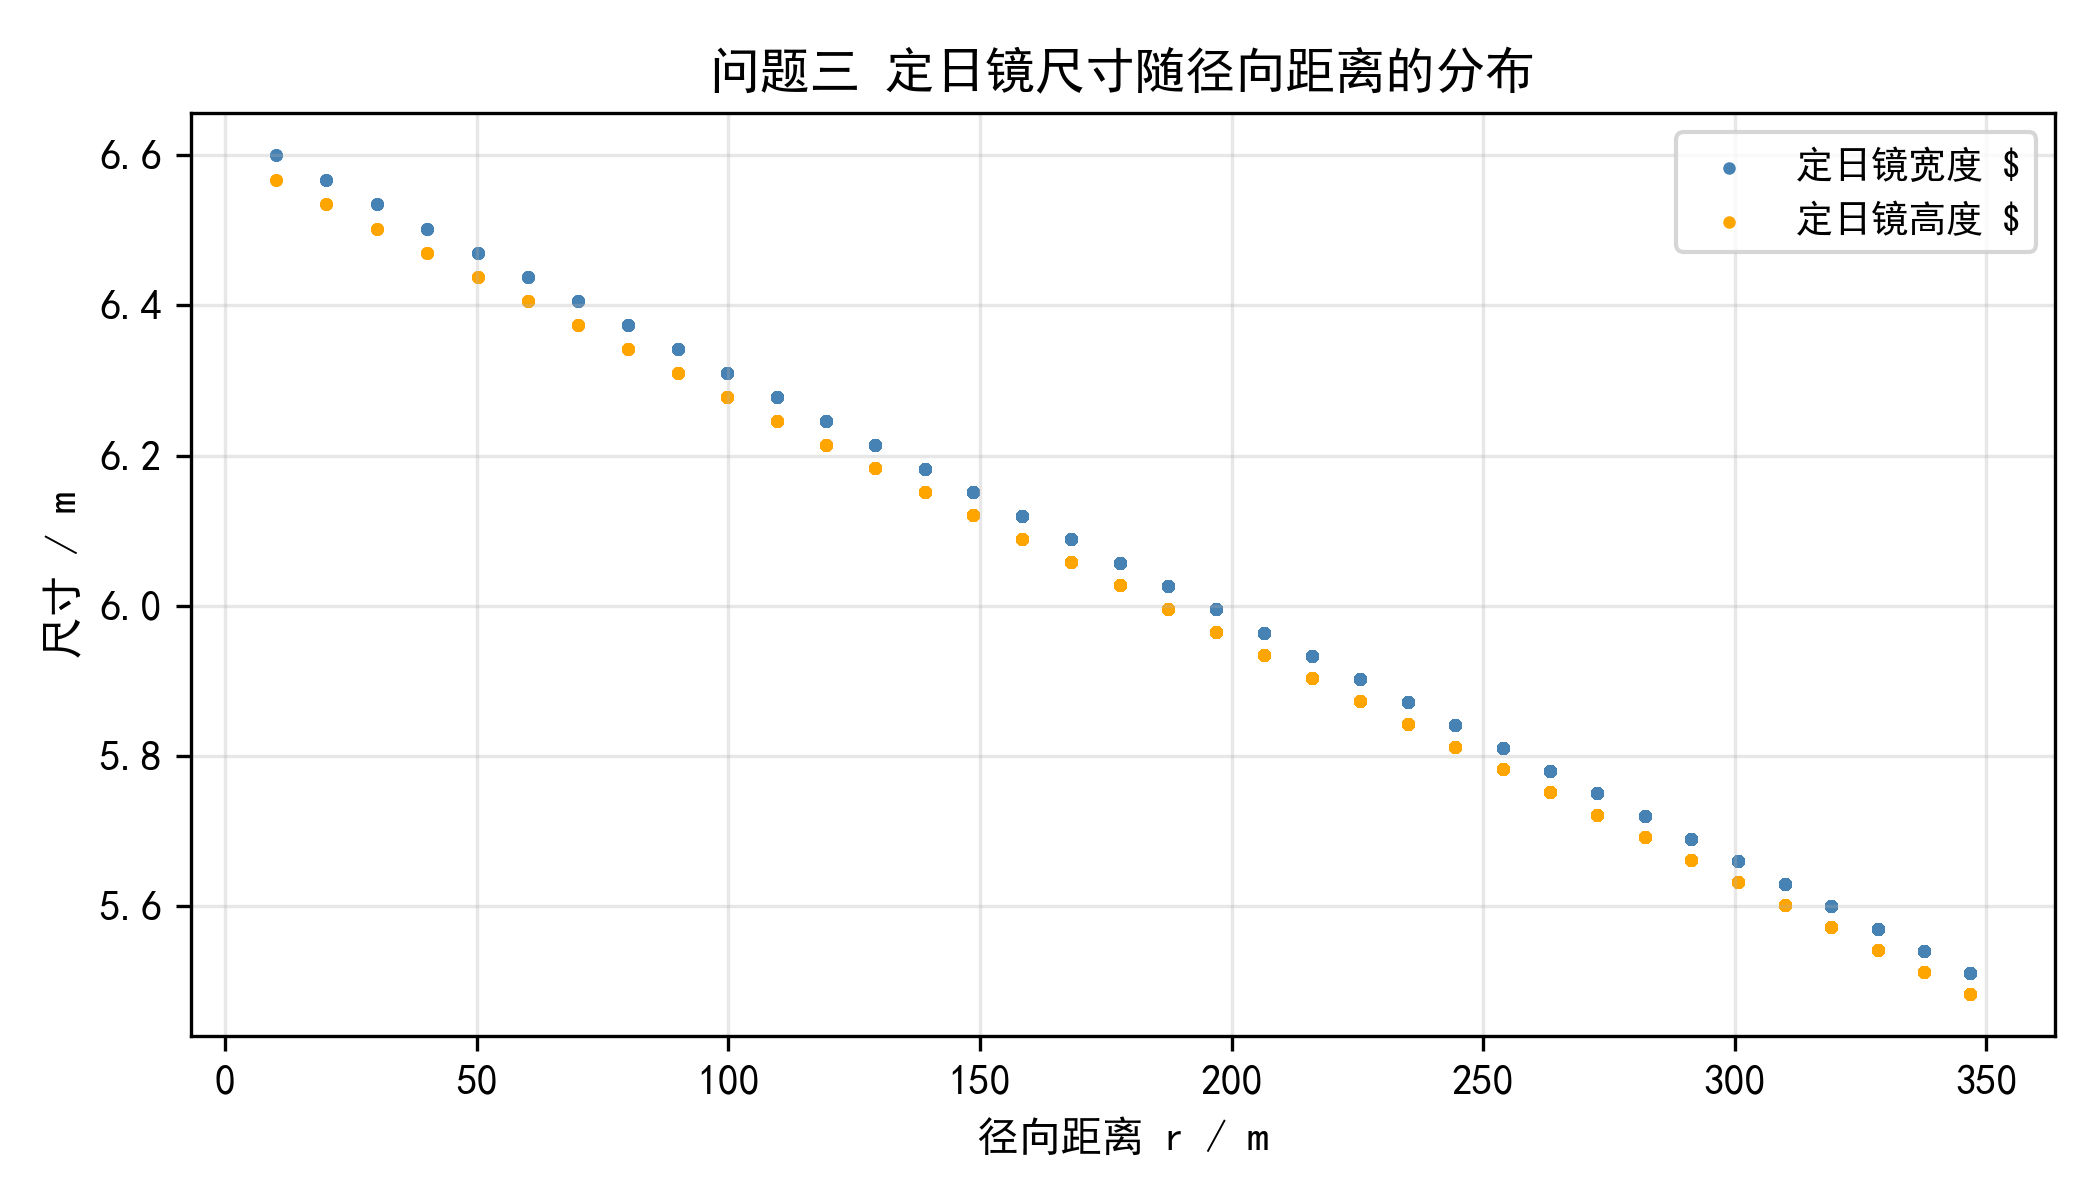
\includegraphics[width=0.75\textwidth]{fig10_p3_size.png}
\caption{问题三定日镜尺寸随径向距离的分布}
\label{fig:fig10_p3_size}
\end{figure}

安装高度同样允许差异化。安装高度通过两条途径影响效率：一是改变镜面到集热器的距离（影响大气透射率与截断效率），二是改变镜面离地高度（影响阴影遮挡）。完整光线追踪的高度敏感性验证表明（表~\ref{tab:h_sens}），安装高度由 $2.5$ m 增至 $5.0$ m 时，阴影遮挡效率仅由 $0.755$ 降至 $0.746$，单位面积功率仅变化 $1.5\%$；且安装高度受"镜面绕水平轴旋转时不得触及地面"约束，即 $h\ge H/2$，故最优安装高度取略高于 $H/2$。进一步对"高度随环半径线性变化"的策略进行优化尝试：内环取触地约束下限（$H_{in}/2+0.05\approx3.33$ m），外环安装高度在 $3.5$--$5.0$ m 间扫描，结果表明外环安装高度越高、单位面积功率略高（外环高度由 $3.5$ m 增至 $5.0$ m 时，单位面积功率由 $0.5135$ 增至 $0.5140$ kW/m$^2$，提升约 $0.1\%$），收益极其微小。综合尺寸与高度的分析，问题三的结论是：差异化尺寸（内大外小）可通过提高外环截断效率带来 $1.4\%$ 的单位面积功率提升，而差异化高度仅有约 $0.1\%$ 的微小收益，可近似忽略。

\begin{table}[H]
\centering
\begin{tabular}{lccccc}
\toprule
安装高度 $h$ (m) & 2.5 & 3.15 & 4.0 & 5.0 \\
\midrule
阴影遮挡效率 & 0.755 & 0.753 & 0.749 & 0.746 \\
单位面积功率 (kW/m$^2$) & 0.507 & 0.505 & 0.502 & 0.499 \\
\bottomrule
\end{tabular}
\caption{安装高度敏感性（完整光线追踪）}
\label{tab:h_sens}
\end{table}

三个问题的结果对比如图~\ref{fig:fig6_compare} 所示，关键结果汇总见附录表~\ref{tab:summary}。

\begin{figure}[H]
\centering
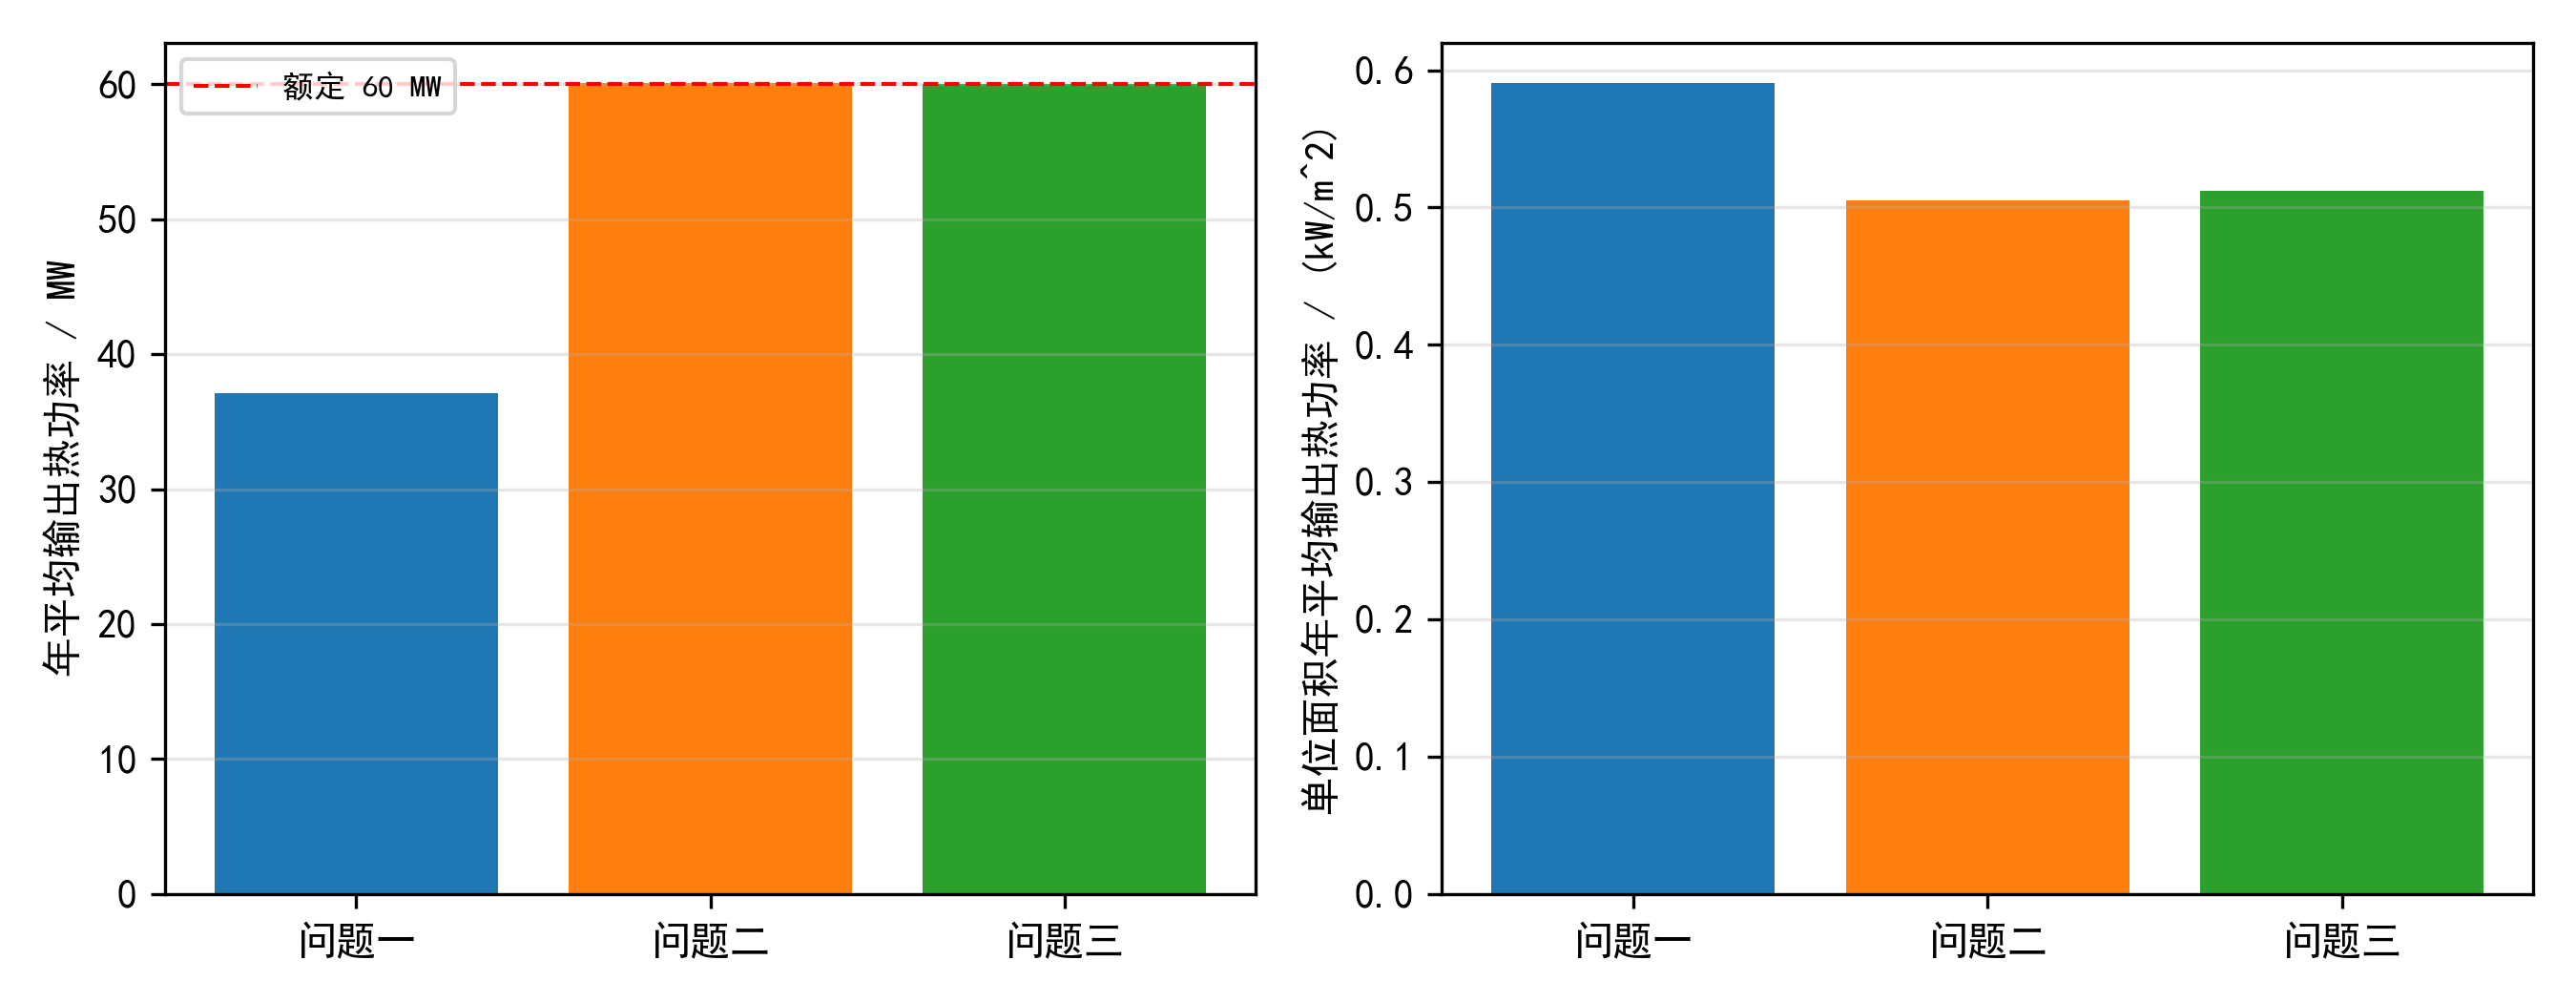
\includegraphics[width=0.95\textwidth]{fig6_compare.png}
\caption{三个问题结果对比}
\label{fig:fig6_compare}
\end{figure}

\section{模型评价与改进}
本文对关键参数进行了系统的灵敏度分析，汇总如下：
\begin{itemize}
\item \textbf{吸收塔纵向位置}（影响最大）：塔由圆心南移 $150$ m，余弦效率由 $0.754$ 升至 $0.823$（变化 $9\%$），是本次优化中收益最大的决策；
\item \textbf{定日镜宽度}：由 $6.0$ m 增至 $6.6$ m，单位面积功率由 $0.498$ 降至 $0.469$（变化 $6\%$），截断损失是主要机制；
\item \textbf{布局间距}：由 $20$ m 减至 $11$ m，阴影遮挡效率由 $0.976$ 降至 $0.784$（变化 $20\%$），但间距增大又会使功率不足。
\end{itemize}
最优解对吸收塔纵向位置较为敏感，但在 $y_t\in[-150,-100]$ m 范围内单位面积功率变化平缓（$0.505$--$0.518$ kW/m$^2$），说明结果具有一定的稳健性。整体而言，吸收塔纵向位置、定日镜尺寸与布局间距三者形成功率与效率的权衡，本文的最优解正是这一权衡的平衡点。

\subsection{模型优点}
\begin{enumerate}
\item 采用蒙特卡洛光线追踪精确计算阴影遮挡与截断效率，物理机理清晰，并通过解析基准模型对比验证了其必要性；
\item 通过阴影遮挡效率的标定建立快速代理模型，在保证精度的同时大幅提升优化效率；
\item 重点识别并利用了吸收塔向南偏移这一关键优化变量，使单位面积功率较圆心方案提升 $4.6\%$；
\item 布局参数化与差分进化算法结合，有效处理了大规模连续优化问题，时间复杂度与镜子数目近似线性，可扩展性强。
\end{enumerate}

\subsection{模型不足与改进}
\begin{enumerate}
\item \textbf{全局最优性}：优化采用代理模型与差分进化（含 L-BFGS-B 局部搜索），但仍可能未达到严格全局最优。可进一步采用多起点策略或贝叶斯优化对最优解进行交叉验证。
\item \textbf{阴影遮挡经验模型}：在塔大幅偏移等非对称布局下存在一定偏差，可扩展为更一般的解析模型或采用逐环标定。
\item \textbf{时间分辨率}：年平均指标仅基于每月 $21$ 日 $5$ 个时点（共 $60$ 个数据点），未能覆盖日内其他时刻与季节内的日际变化。虽然这是题目的简化要求，但采用全年逐时（$8760$ 个时点）数据可更精确地反映年均性能，代价是计算量增大约 $146$ 倍，需借助更高效的并行或代理模型。
\item \textbf{天气因素}：DNI 模型仅依赖太阳高度角与海拔，未考虑云量、气溶胶等动态气象因素。模型向实际工程应用扩展时，需引入当地实测辐射数据或典型气象年（TMY）数据以修正 DNI。
\item \textbf{镜面反射率}：取常数 $0.92$，实际银镜反射率随入射角增大而轻微下降。引入角度依赖的 Fresnel 反射模型需银镜的复折射率（$n,\ k$）数据，该数据依赖镜面镀膜工艺，题目未给定；且本题入射角范围有限（余弦效率 $0.68$--$0.94$，对应入射角约 $20^\circ$--$47^\circ$），在该范围内银镜反射率变化小于 $2\%$，故本文采用常数反射率是合理的简化。
\item \textbf{差异化高度}：本文已给出"高度随环半径变化"的优化尝试，结果表明其收益仅约 $0.1\%$，故在问题三中未将其作为独立决策变量。
\end{enumerate}

\appendix
\section{蒙特卡洛光线追踪算法}
本文计算阴影遮挡与截断效率的核心算法流程如下：

\begin{enumerate}
\item \textbf{几何初始化}：对每个时点，根据太阳方向 $\mathbf{s}$ 与镜面中心 $\mathbf{M}$、集热器中心 $\mathbf{T}$，计算镜面法向 $\mathbf{n}$、镜面局部基 $(\mathbf{u},\mathbf{v})$ 及四顶点坐标。
\item \textbf{采样}：对每面镜子，在镜面矩形内均匀采样 $K$ 个点 $\mathbf{p}$，入射方向在太阳锥内按均匀盘面采样 $\mathbf{s}'$。
\item \textbf{阴影判断}：从 $\mathbf{p}$ 沿 $\mathbf{s}'$ 发射光线，用二维 DDA 遍历均匀网格中的候选镜子，若与任一其他镜子相交则记入阴影。
\item \textbf{遮挡判断}：对未阴影的采样，计算反射方向 $\mathbf{r}'=-\mathbf{s}'+2(\mathbf{s}'\cdot\mathbf{n})\mathbf{n}$，沿 $\mathbf{r}'$ 发射光线判断是否被其他镜子遮挡。
\item \textbf{截断判断}：对未被遮挡的采样，用解析法判断反射光线是否命中集热器圆柱（侧面与上下底）。
\item \textbf{统计}：由阴影数 $n_{sh}$、遮挡数 $n_{bl}$、命中数 $n_{hit}$ 计算 $\eta_{sb}$ 与 $\eta_{trunc}$。
\end{enumerate}

\section{差分进化算法参数}
问题二、三采用的差分进化算法参数设置如下：
\begin{center}
\resizebox{\textwidth}{!}{%
\begin{tabular}{lcccc}
\toprule
参数 & 种群规模 $NP$ & 迭代次数 & 缩放因子 $F$ & 交叉概率 $CR$ \\
\midrule
取值 & 10 & 40 & 0.8 & 0.9 \\
\bottomrule
\end{tabular}%
}
\end{center}

\section{关键数值结果汇总}
\begin{table}[H]
\centering
\resizebox{\textwidth}{!}{%
\begin{tabular}{lccc}
\toprule
指标 & 问题一 & 问题二 & 问题三 \\
\midrule
吸收塔位置 (m) & $(0,0)$ & $(0,-120)$ & $(0,-120)$ \\
定日镜尺寸 (宽$\times$高, m) & $6.0\times6.0$ & $6.0\times5.97$ & 内 $6.6$/外 $5.5$ \\
安装高度 (m) & 4.0 & 3.15 & 内 $3.45$/外 $2.90$ \\
定日镜总面数 & 1745 & 3321 & 3455 \\
定日镜总面积 (m$^2$) & 62820 & 119021 & 117163 \\
年平均光学效率 & 0.607 & 0.519 & 0.519 \\
年平均输出热功率 (MW) & 37.08 & 60.06 & 60.00 \\
单位面积输出热功率 (kW/m$^2$) & 0.590 & 0.505 & 0.512 \\
\bottomrule
\end{tabular}%
}
\caption{三个问题关键结果汇总}
\label{tab:summary}
\end{table}

\begin{thebibliography}{9}
\bibitem{zhang} 张平等. 太阳能塔式光热镜场光学效率计算方法[J]. 技术与市场, 2021, 28(6): 5--8.
\bibitem{cai} 蔡志杰. 太阳影子定位[J]. 数学建模及其应用, 2015, 4(4): 25--33.
\bibitem{du} 杜宇航等. 塔式光热电站定日镜不同聚焦策略的影响分析[J]. 动力工程学报, 2020, 40(5): 426--432.
\bibitem{farges} O. Farges, J.J. Bezian, M. El Hafi. Global optimization of solar power tower systems using a Monte Carlo algorithm: Application to a redesign of the PS10 solar thermal power plant[J]. Renewable Energy, 2018, 119: 345--353.
\end{thebibliography}

\end{document}
